% =========
% CHƯƠNG 6
% =========
\OpenGrid

\ParallelChapter
  {Reasoning with Functions}
  {Luận với hàm số}
  {}

\TriPara
  {
    \EN{Functions are one of the most important mathematical tools for helping students make sense of the world around them, as well as preparing them for further study in mathematics (Yerushalmy and Shternberg 2001). Functions appear in most branches of mathematics and provide a consistent way of making connections between and among topics. Students' continuing development of the concept of function must be rooted in reasoning, and likewise functions are an important tool for reasoning. Thus, developing procedural fluency in using functions is a significant goal of high school mathematics.}
  }
  {
    \VI{Hàm số là một trong những công cụ toán học quan trọng nhất giúp học sinh hiểu thế giới xung quanh, đồng thời chuẩn bị cho các em tiếp tục học toán ở trình độ cao hơn (Yerushalmy and Shternberg 2001). Hàm số xuất hiện trong hầu hết nhánh của toán học và cung cấp cách nhất quán để thiết lập kết nối giữa những chủ đề khác nhau. Quá trình học sinh tiếp tục phát triển khái niệm hàm số phải được đặt nền tảng trên luận; ngược lại, hàm số cũng là công cụ quan trọng để luận. Vì vậy, phát triển thành thạo thủ tục khi sử dụng hàm số là mục tiêu quan trọng của toán học trung học phổ thông.}
  }{\NOTE{}}

\TriPara
  {
  \EN{
  Key elements of reasoning and sense making with functions include the following:

  \begin{itemize}
    \item \emph{Using multiple representations of functions.} Representing functions in various ways, including tabular, graphic, symbolic (explicit and recursive), visual, and verbal; making decisions about which representations are most helpful in problem-solving circumstances; and moving flexibly among those representations.\vspace{\baselineskip}
    
    \item \emph{Modeling by using families of functions.} Working to develop a reasonable mathematical model for a particular contextual situation by applying knowledge of the characteristic behaviors of different families of functions.
    
    \item \emph{Analyzing the effects of parameters.} Using a general representation of a function in a given family (e.g., the vertex form of a quadratic, $f(x) = a(x - h)2 + k$) to analyze the effects of varying coefficients or other parameters; converting between different forms of functions (e.g., the standard form of a quadratic and its factored form) according to the requirements of the problem-solving situation (e.g., finding the vertex of a quadratic or finding its zeros).
  \end{itemize}\vspace{\baselineskip}

  We address these key elements in more detail in the following sections.}
  }
  {
  \VI{
    Các yếu tố then chốt của luận và hiểu với hàm số gồm có:
    \begin{itemize}
      \item \emph{Sử dụng nhiều biểu diễn của hàm số.} Biểu diễn hàm số theo nhiều cách khác nhau, bao gồm bằng bảng, bằng đồ thị, bằng kí hiệu (cả dạng tường minh và dạng truy hồi) bằng hình ảnh và bằng lời; quyết định biểu diễn nào hữu ích nhất trong từng tình huống giải quyết vấn đề; và chuyển đổi linh hoạt giữa các biểu diễn ấy.

      \item \emph{Mô hình hóa bằng các họ hàm số.} Xây dựng mô hình toán học hợp lí cho tình huống có ngữ cảnh cụ thể bằng cách vận dụng hiểu biết về hành vi đặc trưng của những họ hàm số khác nhau.
      
      \item \emph{Phân tích ảnh hưởng của tham số.} Sử dụng biểu diễn tổng quát của hàm số trong một họ đã cho (chẳng hạn dạng đỉnh của hàm số bậc hai, $f(x)=a(x-h)^2+k$) để phân tích ảnh hưởng của việc thay đổi hệ số hoặc tham số khác; chuyển đổi giữa những dạng khác nhau của hàm số (chẳng hạn dạng chuẩn của hàm số bậc hai và dạng phân tích thành nhân tử của nó) tùy theo yêu cầu của tình huống giải quyết vấn đề (chẳng hạn tìm đỉnh của hàm số bậc hai hoặc tìm các không điểm của nó).
    \end{itemize}

    Chúng tôi sẽ trình bày chi tiết hơn các yếu tố then chốt này trong những phần tiếp theo.}
  }{\NOTE{}}

\ParallelSection
  {Using Multiple Representations of Functions}
  {Sử dụng nhiều biểu diễn của hàm số}
  {}

\TriPara
  {
    \EN{Different representations of a function---tables, graphs or diagrams, symbolic expressions, and verbal descriptions---exhibit different properties. Using a variety of representations can help make functions more understandable to a wider range of students than can be accomplished by working with symbolic representations alone (Lloyd and Wilson 1998; Coulombe and Berenson 2001). Students need to establish connections among different representations, for example, the relationship among the zeros of a function, the solution of an equation, and the $x$-intercepts of graphs.}
  }
  {
    \VI{Những biểu diễn khác nhau của hàm số---bảng, đồ thị hoặc sơ đồ, biểu thức kí hiệu, và mô tả bằng lời---làm bộc lộ những tính chất khác nhau. Sử dụng đa dạng biểu diễn có thể giúp nhiều đối tượng học sinh hiểu hàm số tốt hơn so với việc chỉ làm việc với biểu diễn kí hiệu (Lloyd and Wilson 1998; Coulombe and Berenson 2001). Học sinh cần thiết lập kết nối giữa những biểu diễn khác nhau, chẳng hạn mối liên hệ giữa không điểm của hàm số, nghiệm của phương trình, và giao điểm của đồ thị với trục $x$.}
  }{\NOTE{}}

\TriPara
  {
    \EN{Functions whose domains are the natural numbers are often represented recursively, where $f(k + 1)$ is defined in terms of $f(k)$ and an initial function value is given. Such functions can also be presented as sequences, and they are used in applications involving discrete rather than continuous data, often with the support of a calculator or an electronic spreadsheet; see example 10, ``Patterns, Plane and Symbol,'' and example 11, ``Take As Directed.''}
  }
  {
    \VI{Những hàm số có miền xác định là số tự nhiên thường được biểu diễn dưới dạng truy hồi, trong đó $f(k+1)$ được xác định theo $f(k)$ và một giá trị ban đầu của hàm số được cho trước. Những hàm số như vậy cũng có thể được trình bày dưới dạng dãy số, và được dùng trong những ứng dụng liên quan đến dữ liệu rời rạc thay vì dữ liệu liên tục, thường với sự hỗ trợ của máy tính cầm tay hoặc bảng tính điện tử; xem Ví dụ 10, ``Thêm đường thêm miền'', và Ví dụ 11, ``Uống theo chỉ dẫn''.}
  }{\NOTE{}}

\TriPara
  {
    \EN{One interesting exploration is to investigate the number of regions into which a plane is divided by $n$ straight lines. The first question is whether $n$ lines always divide the plane into the same number of regions. Experiments with two or three lines should help students see that different numbers of regions result. For example, two lines that cross create four regions, whereas two parallel lines create only three. Three parallel lines produce four regions; three lines all going through the same point create six regions; but three nonparallel, nonconcurrent lines create seven regions. In general, $n$ parallel lines create only $n + 1$ regions, whereas $n$ lines that all pass through the same point create $2n$ regions. The next example explores what happens in the case of nonparallel, nonconcurrent lines. It could be used with students entering high school, who are beginning to develop the ability to express functional relationships symbolically, or with more advanced students who are working to improve their profi ciency with algebraic manipulation. Example 10 illustrates how students can use various representations of functions, including verbal descriptions, tables, formulas, and various geometric models to make sense of a problem.}
  }
  {
    \VI{Một hướng khám phá thú vị là khảo sát số miền mà mặt phẳng bị chia cắt bởi $n$ đường thẳng. Câu hỏi đầu tiên đặt ra là liệu $n$ đường thẳng luôn chia mặt phẳng thành cùng một số miền hay không. Thử nghiệm với hai hoặc ba đường thẳng sẽ giúp học sinh thấy rằng những cách bố trí khác nhau tạo ra số miền khác nhau. Chẳng hạn, hai đường thẳng cắt nhau tạo ra bốn miền, trong khi hai đường thẳng song song chỉ tạo ra ba miền. Ba đường thẳng song song tạo ra bốn miền; ba đường thẳng cùng đi qua một điểm tạo ra sáu miền; còn ba đường thẳng không song song và không đồng quy tạo ra bảy miền. Nói chung, $n$ đường thẳng song song chỉ tạo ra $n+1$ miền, trong khi $n$ đường thẳng cùng đi qua một điểm tạo ra $2n$ miền. Ví dụ tiếp theo khảo sát điều xảy ra trong trường hợp không có hai đường thẳng nào song song và không có quá hai đường thẳng cùng đi qua một điểm. Ví dụ này có thể được dùng với học sinh mới vào trung học phổ thông, khi các em bắt đầu phát triển khả năng biểu diễn quan hệ hàm số bằng kí hiệu, hoặc với học sinh ở trình độ cao hơn đang rèn luyện thành thạo biến đổi đại số. Ví dụ 10 minh họa cách học sinh có thể sử dụng nhiều biểu diễn khác nhau của hàm số, bao gồm mô tả bằng lời, bảng, công thức và mô hình hình học khác nhau, để hiểu một bài toán.}
  }{\NOTE{}}

\TriExample
  {
    \small\mbox{Patterns, Plane and Symbol}
  }
  {
    \textbf{Task}

    Develop a symbolic representation for a function that produces the number of regions in a plane formed by intersecting lines such that no two lines are parallel and no more than two lines intersect in the same point, as shown in the figure.

    \begin{center}
      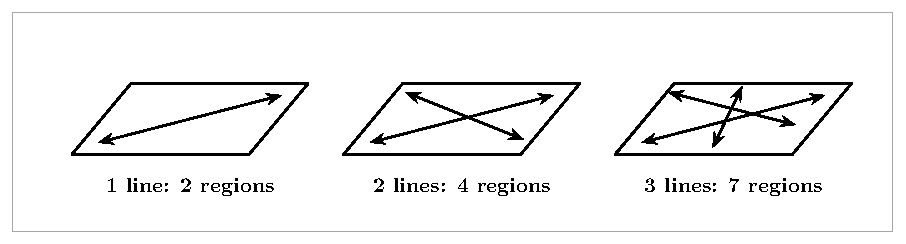
\includegraphics[width=.92\linewidth]{../figures/fhsm_2009_p42_f1_en.pdf}
    \end{center}

    \textbf{In the Classroom}

    Students may approach this problem in several different ways, depending on their level of mathematical experience.

    \begin{description}
      \item[Method 1.] After exploring a number of cases, possibly using an interactive geometry tool, students may produce a table of values for the number of lines, $L$, and the number of regions, $R$, as shown here:
        \begin{center}
        \setlength{\tabcolsep}{4pt}
        \begin{tabular}{|l|c|c|c|c|c|c|}
        \hline
        \shortstack[l]{No. of lines ($L$)} 
          & $1$ & $2$ & $3$ & $4$ & $5$ & $6$ \\
        \hline
        \shortstack[l]{No. of regions ($R$)} 
          & $2$ & $4$ & $7$ & $11$ & $16$ & $22$ \\
        \hline
        \end{tabular}
        \end{center}
      Students commonly observe the pattern of differences between consecutive terms of a sequence. This observation lends itself to a recursive definition of a function. In this example, a recursive definition would be $R(1) = 2, R(L) = R(L - 1) + L$.

      \item[Method 2.] An interesting geometric approach to helping students reason about this problem is to use checkers, coins, tiles, or other small objects to create a pattern in which the value of $L$ defines the number of rows of objects and the value of $R$ defines the total number of objects in the figure, as shown in the following sequence:
      
        \begin{center}
          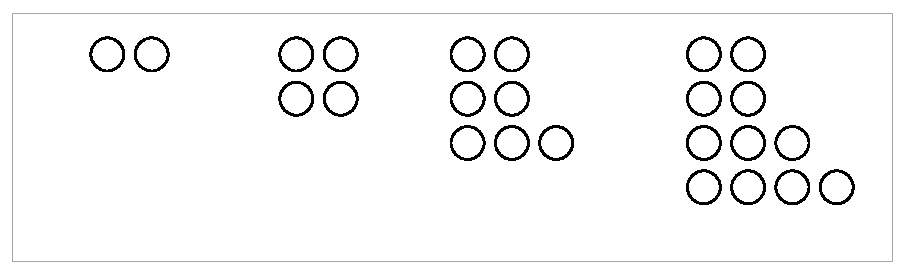
\includegraphics[width=.92\linewidth]{../figures/fhsm_2009_p43_1.pdf}
        \end{center}

      Removing one of the objects from the top row results in a triangular pattern, as shown below:
        
        \begin{center}
          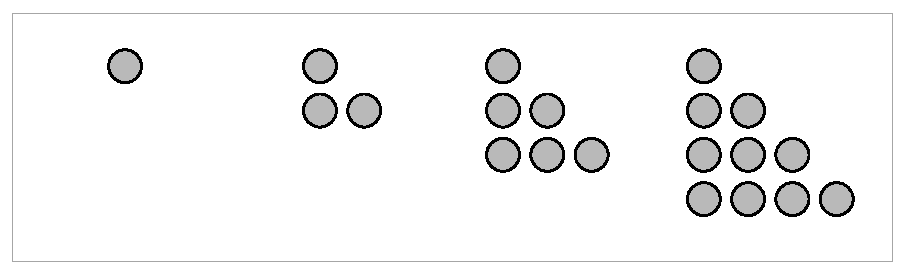
\includegraphics[width=.92\linewidth]{../figures/fhsm_2009_p43_2.pdf}
        \end{center}
      
      Doubling and transforming this pattern can result in a rectangle containing $L(L + 1)$ objects, as shown here:

        \begin{center}
          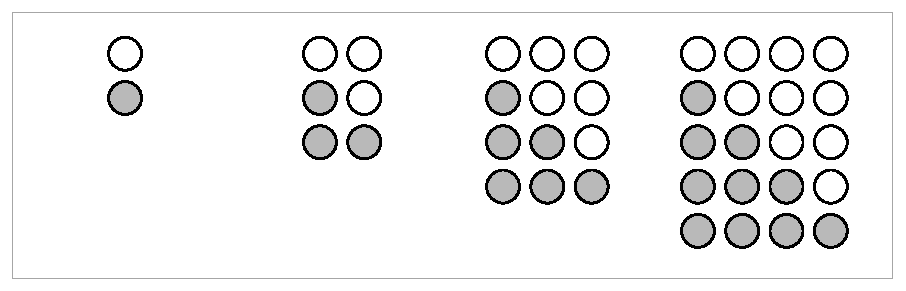
\includegraphics[width=.92\linewidth]{../figures/fhsm_2009_p43_3.pdf}
        \end{center}

      From this configuration, one can see that the original objects, minus the one that was removed, form half the rectangle. The explicit definition of this function can then be written as
      $$
      R=\frac{1}{2}(L)(L+1)+1=\frac{1}{2}L^2+\frac{1}{2}L+1.
      $$

      This type of approach demonstrates how a student who is given the opportunity to represent a function pictorially can use a simple geometric pattern to write the explicit definition of the function. The student can then extend his or her reasoning about symbolic representations by developing it from a familiar starting place.

      \item[Method 3.] By applying technology to numeric and graphical reasoning, students may enter a number of ordered pairs from the table into a graphing calculator and examine a scatterplot of the pairs to conjecture that the relationship is quadratic because of the parabolic shape of the graph. On the basis of that conjecture, students could use calculator-assisted quadratic regression to find the function $R = 0.5L^2 + 0.5L + 1$. This algebraic model could be tested by using ordered pairs from the table.
      
      \item[Method 4.] The teacher could ask students to focus on the differences between consecutive terms of the sequence of R values: $2, 3, 4, 5,$ and so forth. By applying algebraic reasoning, students may examine the data and observe that the function is quadratic because the first differences are linear so the second differences are constant. The geometric representation shown in part 1 of this example can be used to reinforce this concept for students. Writing a system of equations of the form $R = aL^2 + bL + c$, substituting three ordered pairs, and solving the system would reveal that
      $$
        \begin{aligned}
          a=\frac{1}{2}, \; b=\frac{1}{2}, \; \text{and} \; c=1; \; \text{thus}\\
          R=\frac{1}{2}L^2+\frac{1}{2}L+1.
        \end{aligned}
      $$

      This strategy would require a sophisticated understanding of several mathematical topics and a command of algebraic manipulation developed later in the high school experience.
    \end{description}

    \textbf{Key Elements of Mathematics}

    \begin{hanglist}
      \hangitem{Reasoning with Functions---Using multiple representations of functions}
      \hangitem{Reasoning with Algebraic Symbols---Connecting algebra with geometry; Linking expressions and functions}
    \end{hanglist}

    \textbf{Reasoning Habits}

    \begin{hanglist}
      \hangitem{Analyzing a problem---seeking patterns and relationships}
      \hangitem{Seeking and using connections}
      \hangitem{Reflecting on a solution---justifying or validating a solution}
    \end{hanglist}
  }
  {
    Thêm đường thêm miền
  }
  {
    \textbf{Nhiệm vụ}

    Hãy xây dựng biểu diễn kí hiệu cho hàm số cho biết số miền của mặt phẳng được tạo thành bởi các đường thẳng cắt nhau sao cho không có hai đường thẳng nào song song và không có quá hai đường thẳng cùng đi qua một điểm, như trong hình vẽ.

    \begin{center}
      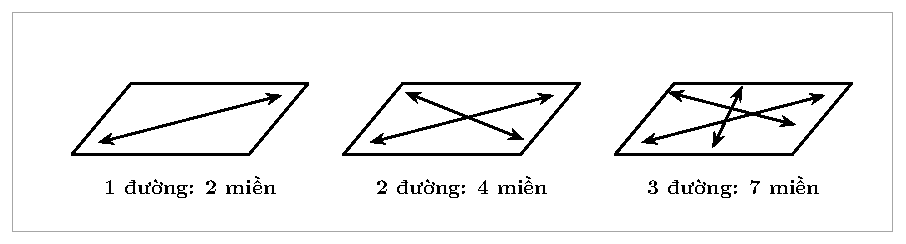
\includegraphics[width=.92\linewidth]{../figures/fhsm_2009_p42_f1_vi.pdf}
    \end{center}

    \textbf{Trong lớp học}

    Học sinh có thể tiếp cận bài toán này theo nhiều cách khác nhau, tùy thuộc vào mức độ trải nghiệm toán học của các em.

    \begin{description}
      \item[Phương pháp 1.] Sau khi khảo sát một số trường hợp, có thể với sự hỗ trợ của công cụ hình học tương tác, học sinh có thể lập bảng giá trị cho số đường thẳng $L$ và số miền $R$, như sau:\vspace{\baselineskip}
        \begin{center}
        \setlength{\tabcolsep}{4pt}
        \begin{tabular}{|l|c|c|c|c|c|c|}
        \hline
        \shortstack[l]{Số đường ($L$)} 
          & $1$ & $2$ & $3$ & $4$ & $5$ & $6$ \\
        \hline
        \shortstack[l]{Số miền ($R$)} 
          & $2$ & $4$ & $7$ & $11$ & $16$ & $22$ \\
        \hline
        \end{tabular}
        \end{center}
      Học sinh thường nhận ra mẫu hình của hiệu giữa các số hạng liên tiếp trong một dãy. Quan sát này tự nhiên dẫn tới định nghĩa truy hồi của hàm số. Trong ví dụ này, định nghĩa truy hồi có thể là $R(1)=2,\, R(L)=R(L-1)+L$.\vspace{\baselineskip}

      \item[Phương pháp 2.] Một cách tiếp cận hình học thú vị để giúp học sinh luận về bài toán này là dùng quân cờ, đồng xu, mảnh ghép, hoặc vật nhỏ khác để tạo ra một mẫu hình trong đó giá trị $L$ xác định số hàng các vật, còn giá trị của $R$ xác định tổng số vật trong hình, như trong dãy hình sau:
      
        \begin{center}
          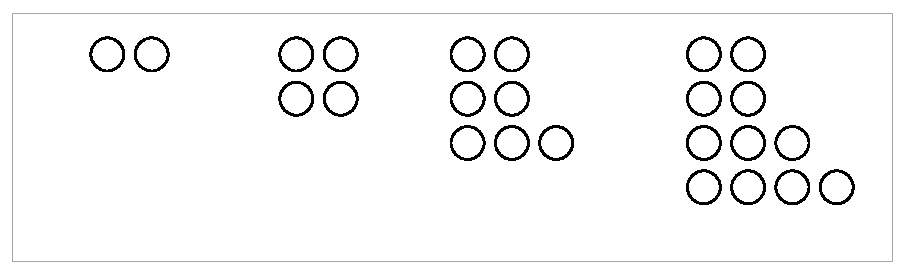
\includegraphics[width=.92\linewidth]{../figures/fhsm_2009_p43_1.pdf}
        \end{center}

      Lấy bớt một vật ở hàng trên cùng sẽ tạo ra mẫu hình tam giác, như minh họa dưới đây:
        
        \begin{center}
          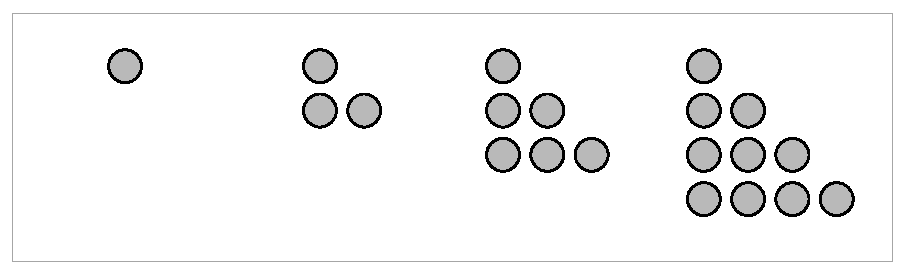
\includegraphics[width=.92\linewidth]{../figures/fhsm_2009_p43_2.pdf}
        \end{center}
      
      Nhân đôi và biến đổi mẫu hình này có thể tạo thành hình chữ nhật chứa $L(L+1)$ vật, như sau:

        \begin{center}
          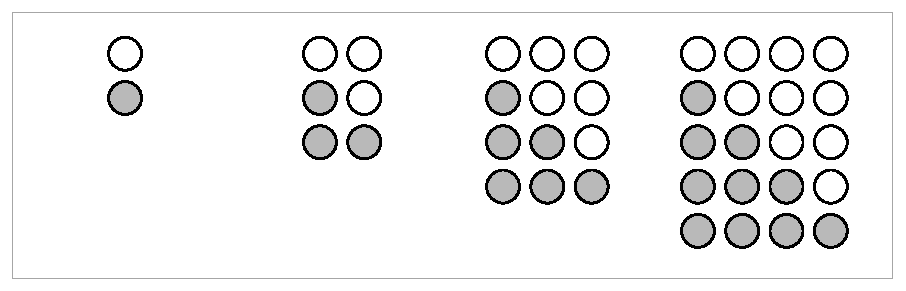
\includegraphics[width=.92\linewidth]{../figures/fhsm_2009_p43_3.pdf}
        \end{center}

      Từ cấu hình này, có thể thấy các vật ban đầu còn lại sau khi lấy bớt một vật tạo thành một nửa hình chữ nhật. Khi đó, công thức tường minh của hàm số có thể được viết là
      $$
      R=\frac{1}{2}(L)(L+1)+1=\frac{1}{2}L^2+\frac{1}{2}L+1.
      $$

      Kiểu tiếp cận này cho thấy học sinh khi có cơ hội biểu diễn hàm số bằng hình ảnh có thể dùng mẫu hình hình học đơn giản để viết ra công thức tường minh của hàm số. Từ đó, học sinh có thể mở rộng luận của mình về các biểu diễn kí hiệu bằng cách phát triển luận ấy từ một điểm khởi đầu quen thuộc.\vspace{\baselineskip}

      \item[Phương pháp 3.] Bằng cách dùng công nghệ để hỗ trợ luận bằng số và bằng đồ thị, học sinh có thể nhập một số cặp có thứ tự từ bảng vào máy tính vẽ đồ thị và quan sát biểu đồ phân tán của các cặp điểm để phỏng đoán rằng quan hệ này là bậc hai vì đồ thị có dạng parabol. Từ phỏng đoán ấy, học sinh có thể dùng phép hồi quy bậc hai với sự hỗ trợ của máy tính để tìm hàm số $R=0.5L^2+0.5L+1$. Mô hình đại số này có thể được kiểm tra bằng cách dùng các cặp có thứ tự trong bảng.\vspace{\baselineskip}
      
      \item[Phương pháp 4.] Giáo viên có thể yêu cầu học sinh tập trung vào hiệu giữa các số hạng liên tiếp của dãy giá trị $R$: $2, 3, 4, 5$, vân vân. Bằng cách vận dụng luận đại số, học sinh có thể xem xét dữ liệu và nhận ra rằng hàm số là bậc hai vì sai phân bậc nhất là tuyến tính nên sai phân bậc hai là hằng số. Biểu diễn hình học ở phần 1 của ví dụ này có thể được dùng để củng cố ý tưởng ấy cho học sinh. Viết hệ phương trình có dạng $R=aL^2+bL+c$, thế ba cặp có thứ tự vào rồi giải hệ sẽ cho thấy rằng\vspace{2\baselineskip}
      $$
        \begin{aligned}
          a=\frac{1}{2}, \; b=\frac{1}{2}, \; \text{và} \; c=1; \; \text{do đó}\\
          R=\frac{1}{2}L^2+\frac{1}{2}L+1.
        \end{aligned}
      $$
      Chiến lược này đòi hỏi sự hiểu biết tinh vi về nhiều chủ đề toán học và khả năng thành thạo biến đổi đại số thường chỉ được phát triển ở giai đoạn muộn hơn của trung học phổ thông.
    \end{description}

    \textbf{Các yếu tố then chốt của toán học}

    \begin{hanglist}
      \hangitem{Luận với hàm số---Sử dụng nhiều biểu diễn của hàm số}

      \hangitem{Luận với kí hiệu đại số---Kết nối đại số với hình học; Liên kết biểu thức và hàm số}\vspace{\baselineskip}
    \end{hanglist}

    \textbf{Thói quen luận}

    \begin{hanglist}
      \hangitem{Phân tích bài toán---tìm kiếm mẫu hình và quan hệ}

      \hangitem{Tìm kiếm và sử dụng kết nối}

      \hangitem{Phản tư về lời giải---biện minh hoặc kiểm chứng lời giải}
    \end{hanglist}
  }
  {
    \vspace{.5\baselineskip}
    Ví dụ này đáng chú ý vì cùng một bài toán có thể được tiếp cận bằng nhiều con đường khác nhau: bảng số liệu, mô hình hình học, đồ thị - hồi quy và sai phân đại số. Các con đường ấy đều dẫn đến cùng công thức
    $$
      R=\frac12L^2+\frac12L+1,
    $$
    nhưng mỗi con đường giúp người học hiểu công thức này theo một cách riêng: như một quy luật truy hồi, một cấu trúc hình học, một mô hình bậc hai khớp với dữ liệu, hoặc kết quả của một quy luật sai phân.

    Nguồn gốc của Phương pháp 2 thực ra đã xuất hiện từ Phương pháp 1. Từ bảng giá trị, học sinh thấy rằng số miền không tăng đều, mà tăng thêm lần lượt $2,3,4,5,\dots$ khi mỗi đường mới được thêm vào. Điều đó cho thấy số miền sau $L$ đường có thể được hiểu như kết quả của một quá trình cộng dồn. Phương pháp 2 làm cho cấu trúc cộng dồn ấy hiện ra dưới dạng hình ảnh: $R$ được biểu diễn bằng tổng số vật; bỏ đi $1$ vật ở hàng trên cùng thì phần còn lại tạo thành một mẫu tam giác; gấp đôi mẫu ấy rồi ghép lại thì được một hình chữ nhật có $L(L+1)$ vật. Vì thế, phần còn lại sau khi bỏ đi $1$ vật chiếm đúng một nửa hình chữ nhật, nên
    $$
      R-1=\frac{L(L+1)}{2}.
    $$

    Điều đáng chú ý ở đây là công thức tường minh không được đưa ra như một mẹo, mà được rút ra từ một cấu trúc hình học nhìn thấy được.

    Phương pháp 3 đi theo một logic khác. Trước hết, học sinh nhập các cặp dữ liệu
    $$
      (1,2),\, (2,4),\, (3,7),\, (4,11),\, (5,16),\, (6,22)
    $$
    vào máy tính vẽ đồ thị và quan sát biểu đồ phân tán. Hình dạng các điểm gợi ra một parabol, nên học sinh phỏng đoán rằng quan hệ giữa $L$ và $R$ có thể được mô hình hóa bởi một hàm bậc hai. Khi đó, phép hồi quy bậc hai không tự nó ``phát hiện chân lí toán học``, mà hoạt động trong một họ hàm đã được chọn trước:
    $$
      R=aL^2+bL+c.
    $$

    Máy tính sẽ tìm các hệ số $a,b,c$ sao cho tổng bình phương sai lệch giữa giá trị thực tế và giá trị mô hình dự đoán là nhỏ nhất, tức là làm nhỏ nhất biểu thức
    $$
      \sum \left(R_i-(aL_i^2+bL_i+c)\right)^2.
    $$

    Trong ví dụ này, kết quả hồi quy cho
    $$
      R=0.5L^2+0.5L+1.
    $$

    Kiểm tra lại trên các điểm dữ liệu đã cho:
    \begin{align*}
      R(1)&=0.5+0.5+1=2,\\
      R(2)&=2+1+1=4,\\
      R(3)&=4.5+1.5+1=7,\\
      R(4)&=8+2+1=11,\\
      R(5)&=12.5+2.5+1=16,\\
      R(6)&=18+3+1=22.
    \end{align*}

    Vậy các sai lệch đều bằng $0$, nên mô hình bậc hai này khớp hoàn toàn với sáu điểm dữ liệu trong bảng. Tuy nhiên, cần nhấn mạnh rằng hồi quy bậc hai chỉ xác nhận rằng một hàm bậc hai khớp với dữ liệu đã quan sát trong họ mô hình đang xét. Tự nó chưa phải là chứng minh rằng công thức ấy đúng với mọi số đường thẳng $L$. Muốn có kết luận tổng quát, vẫn cần một lập luận toán học khác, chẳng hạn lập luận hình học về cách mỗi đường mới cắt các đường cũ và tạo thêm miền mới.

    Phương pháp 4 làm rõ hơn vì sao dạng bậc hai xuất hiện. Từ bảng dữ liệu
    $$
      \begin{array}{|c|c|c|c|c|c|c|}
      \hline
      L & 1 & 2 & 3 & 4 & 5 & 6\\
      \hline
      R & 2 & 4 & 7 & 11 & 16 & 22\\
      \hline
      \end{array}
    $$
    ta tính sai phân bậc nhất:
    $$
    4-2=2,\, 7-4=3,\, 11-7=4,\, 16-11=5,\, 22-16=6.
    $$

    Vậy dãy sai phân bậc nhất là
    $$
        2,\, 3,\, 4,\, 5,\, 6.
    $$

    Dãy này tăng đều, nên không có gì đáng ngạc nhiên khi sai phân bậc hai là
    $$
        3-2=1,\, 4-3=1,\, 5-4=1,\, 6-5=1.
    $$

    Nói rằng ``sai phân bậc hai không đổi thì hàm là bậc hai`` không nên chỉ được xem như một quy tắc thuộc lòng. Có thể thấy điều này trực tiếp từ biểu thức đại số. Nếu
    $$
        R(L)=aL^2+bL+c,
    $$
    thì sai phân bậc nhất là
    \begin{align*}
        R(L)-&R(L-1)\\
            &=\left(aL^2+bL+c\right)-\left(a(L-1)^2+b(L-1)+c\right)\\
            &=a\left(L^2-(L-1)^2\right)+b\\
            &=a(2L-1)+b\\
            &=2aL+(b-a).
    \end{align*}

    Vậy sai phân bậc nhất của một hàm bậc hai là một hàm tuyến tính theo $L$. Lấy sai phân thêm một lần nữa:
    $$
      \left(R(L)-R(L-1)\right)-\left(R(L-1)-R(L-2)\right)=2a,
    $$
    là một hằng số. Do đó, với hàm bậc hai, sai phân bậc hai luôn không đổi.

    Chiều ngược lại cũng giúp học sinh hiểu sâu hơn. Nếu sai phân bậc hai không đổi, thì sai phân bậc nhất tăng đều; mà cộng dồn một dãy tăng đều sẽ tạo ra một biểu thức bậc hai. Trong dữ liệu của ví dụ này, sai phân bậc nhất là
    $$
        2,\, 3,\, 4,\, 5,\, 6
    $$
    nên có thể đọc được
    \begin{align*}
        R(2)&=R(1)+2,\\
        R(3)&=R(2)+3,\\
        R(4)&=R(3)+4,\\
        R(5)&=R(4)+5,
    \end{align*}
    và nói chung,
    $$
        R(L)=R(L-1)+L.
    $$

    Bắt đầu từ $R(1)=2$, ta có
    $$
        R(L)=2+2+3+\cdots+L.
    $$

    Mà
    $$
        2+3+\cdots+L=(1+2+\cdots+L)-1,
    $$
    nên
    \begin{align*}
        R(L)
        &=2+\left(\frac{L(L+1)}{2}-1\right)\\
        &=\frac{L(L+1)}{2}+1\\
        &=\frac12L^2+\frac12L+1.
    \end{align*}

    Như vậy, sai phân bậc hai không đổi không chỉ là dấu hiệu hình thức để nhận ra hàm bậc hai; nó phản ánh một cấu trúc tăng trưởng: lượng tăng của $R$ không cố định, nhưng chính lượng tăng ấy lại tăng đều.

    Nếu đi đúng theo con đường đại số mà FHSM gợi ý, sau khi nhận ra dữ liệu có dạng bậc hai, ta đặt
    $$
      R=aL^2+bL+c.
    $$

    Thay ba cặp dữ liệu, chẳng hạn $(1,2)$, $(2,4)$ và $(3,7)$, vào đó, ta được hệ
    \begin{align*}
        a+b+c&=2,\\
        4a+2b+c&=4,\\
        9a+3b+c&=7.
    \end{align*}

    Lấy phương trình thứ hai trừ phương trình thứ nhất:
    $$
      3a+b=2.
    $$

    Lấy phương trình thứ ba trừ phương trình thứ hai:
    $$
      5a+b=3.
    $$

    Trừ tiếp hai phương trình này cho nhau:
    $$
        2a=1,\, a=\frac12.
    $$

    Thế lại vào $3a+b=2$, ta được
    $$
        \frac32+b=2,\, b=\frac12.
    $$

    Cuối cùng, từ $a+b+c=2$, suy ra
    $$
        \frac12+\frac12+c=2,\, c=1.
    $$

    Vậy
    $$
        R=\frac12L^2+\frac12L+1.
    $$

    Nhìn như vậy, Phương pháp 4 không phải một mẹo đại số khó hiểu. Nó đi từ bảng dữ liệu, tính sai phân để nhận ra cấu trúc tăng trưởng, rồi từ cấu trúc ấy suy ra công thức hàm số. Tuy nhiên, cần phân biệt rõ giữa việc tìm được một công thức rất có cơ sở và việc chứng minh công thức ấy đúng cho bài toán ban đầu. Bảng giá trị chỉ cho ta dữ liệu hữu hạn; hồi quy bậc hai cho ta một mô hình khớp với dữ liệu đã quan sát; sai phân giúp giải thích vì sao dạng bậc hai là hợp lí; còn mô hình hình học trong Phương pháp 2 giúp công thức tường minh trở nên nhìn thấy được. Nhưng tất cả những điều đó vẫn cần được nối lại với cấu trúc hình học của các đường thẳng chia mặt phẳng.

    Chứng minh nằm ở cơ chế thêm đường. Giả sử đã có $L-1$ đường thẳng thỏa mãn điều kiện không có hai đường nào song song và không có ba đường nào đồng quy. Khi thêm đường thẳng thứ $L$, đường này cắt $L-1$ đường cũ tại $L-1$ điểm phân biệt. Các điểm ấy chia đường thẳng mới thành $L$ phần. Mỗi phần nằm trong một miền cũ và chia miền ấy thành hai miền, nên mỗi phần tạo thêm đúng một miền mới. Do đó, đường thẳng thứ $L$ tạo thêm đúng $L$ miền, tức là
    $$
      R(L)=R(L-1)+L.
    $$

    Với $R(1)=2$, cộng dồn các lượng tăng cho ta
    \begin{align*}
      R(L)
        &=2+2+3+\cdots+L\\
        &=\frac{L(L+1)}{2}+1\\
        &=\frac{1}{2}L^2+\frac{1}{2}L+1.
    \end{align*}

    Vì vậy, hồi quy giúp phỏng đoán và kiểm tra dữ liệu, sai phân giúp giải thích dạng bậc hai, biểu diễn hình học giúp công thức trở nên có nghĩa, nhưng lập luận về đường thẳng thứ $L$ mới là phần chứng minh công thức đúng cho mọi $L$. Đây cũng là điểm sư phạm quan trọng của ví dụ: trong toán học, nhận ra mẫu hình là bước mở đường, còn chứng minh là bước nối mẫu hình ấy với cấu trúc tất yếu của bài toán.

    Điểm sư phạm của Ví dụ 10 không nằm ở việc làm cho lời giải dài hơn một chứng minh ngắn. Nếu đã nhìn ra rằng đường thẳng thứ $L$ cắt $L-1$ đường cũ tại $L-1$ điểm phân biệt, nên bị chia thành $L$ phần và tạo thêm đúng $L$ miền, thì công thức truy hồi $R(L)=R(L-1)+L$ và công thức tường minh theo sau không khó. Nhưng vấn đề của học sinh thường nằm trước bước chứng minh: làm thế nào để nhìn ra cấu trúc ấy, thấy vì sao công thức có dạng như vậy, và hiểu nó từ nhiều biểu diễn khác nhau. Vì thế, các phương pháp trong ví dụ không nhằm thay thế chứng minh, mà nhằm chuẩn bị cho chứng minh trở nên có nghĩa. Bảng số liệu làm lộ mẫu hình tăng trưởng; mô hình hình học làm công thức hiện ra bằng hình ảnh; hồi quy giúp nhận diện dạng bậc hai; sai phân giải thích vì sao dạng bậc hai là hợp lí. Sau đó, lập luận về đường thẳng thứ $L$ mới nối những nhận ra ấy với cấu trúc tất yếu của bài toán và hoàn tất chứng minh.
  }

\ParallelSection
  {Modeling by Using Families of Functions}
  {Mô hình hóa bằng các họ hàm số}
  {}

\TriPara
  {
    \EN{According to \emph{Curriculum Focal Points} (NCTM 2006a), students should enter high school having had extensive experience with linear functions and some exposure to nonlinear functions. High school experiences can help students build on this knowledge and work with parameterized families of functions (e.g., linear, quadratic, exponential, and periodic), each of which has distinguishing characteristics common to all members of the family. Given data from a problem situation, students should be able to (a) choose a family of functions that sensibly models the situation; (b) find parameters for a function to approximately match the data; (c) use the resulting function to solve the problem; and (d) interpret and reflect on their solution in the context of the problem.}
  }
  {
    \VI{Theo \emph{Curriculum Focal Points} (NCTM 2006a), khi bước vào trung học phổ thông, học sinh được kì vọng đã có nhiều trải nghiệm với hàm tuyến tính và đã làm quen phần nào với hàm phi tuyến. Những trải nghiệm học tập ở bậc trung học phổ thông có thể giúp học sinh phát triển trên nền tảng ấy và làm việc với các họ hàm số có tham số (chẳng hạn hàm tuyến tính, hàm bậc hai, hàm mũ và hàm tuần hoàn), trong đó mỗi họ đều có những đặc trưng giúp phân biệt họ đó với các họ khác và được mọi hàm số trong họ chia sẻ. Khi được cung cấp dữ liệu từ một tình huống bài toán, học sinh cần có khả năng: (a) chọn một họ hàm số mô hình hóa tình huống ấy một cách hợp lí; (b) tìm tham số cho một hàm số sao cho khớp xấp xỉ với dữ liệu; (c) sử dụng hàm số thu được để giải bài toán; cùng với (d) diễn giải và phản tư về lời giải của mình trong bối cảnh bài toán.}
  }{\NOTE{}}

\TriPara
  {
    \EN{Using problems that can be extended and revisited as students mature is a powerful way to help students make connections between existing knowledge and new learning. Example 11 uses a context to which students can readily relate and demonstrates how a problem can be extended as students' mathematical backgrounds become more sophisticated. It also shows the power of deductive reasoning in developing a general solution to a problem.}
  }
  {
    \VI{Sử dụng những bài toán có thể mở rộng và quay lại khai thác khi học sinh trưởng thành hơn về mặt toán học là một cách hiệu quả để giúp các em kết nối kiến thức đã có với nội dung học tập mới. Ví dụ 11 sử dụng bối cảnh mà học sinh dễ liên hệ và minh họa cách một bài toán có thể được mở rộng khi nền tảng toán học của các em trở nên sâu sắc hơn. Ví dụ này cũng cho thấy sức mạnh của luận suy diễn trong việc xây dựng lời giải tổng quát cho một bài toán.}
  }{\NOTE{}}

% ----------
% VÍ DỤ 11
% ----------

\TriExample
  {
    Take As Directed
  }
  {
    \textbf{Task}

    A student strained her knee in an intramural volleyball game, and her doctor has prescribed an anti-inflammatory drug to reduce the swelling. The student takes two $220$ mg tablets every $8$ hours for 10 days. Her kidneys eliminate $60$ percent of this drug from her body every $8$ hours. Determine how much of the drug is in her system after $10$ days, just after she takes her last dose of medicine. Explain what happens to the change in the amount of medicine in the body as time progresses and why this pattern occurs. If she continued to take the drug for a year, how much of the drug would be in her system just after she took her last dose? Explain, in mathematical terms and in terms of body metabolism, why the long-term amount of medicine in the body is reasonable (adapted from NCTM [2000b]).

    \textbf{In the Classroom (Variety of Levels from First-Year to Fourth-Year Mathematics)}

    Students may examine this problem in varying degrees of depth, depending on their level of mathematical experience:

    \begin{description}
      \item[Method 1.] Students who are near the beginning of their high school experience could produce a table of data and generate a discrete graph of the data. The following table and graph show the amount of medicine, $A_n$, in mg, in the athlete's body just after taking $n$ doses of medicine.
      
      \begin{center}
      \setlength{\tabcolsep}{5pt}
      \begin{tabular}{|c|c|c|c|c|}
      \hline
      $n$   & $1$      & $2$      & $3$      & $4$      \\
      \hline
      $A_n$ & $440$    & $616$    & $686.40$ & $714.56$ \\
      \hline
      $n$   & $5$      & $6$      & $7$      & $8$      \\
      \hline
      $A_n$ & $725.82$ & $730.33$ & $732.13$ & $732.85$ \\
      \hline
      $n$   & $9$      & $10$     & $11$     & $12$     \\
      \hline
      $A_n$ & $733.14$ & $733.26$ & $733.30$ & $733.32$ \\
      \hline
      $n$   & $\dots$  & $20$     & $\dots$  & $30$     \\
      \hline
      $A_n$ & $\dots$  & $733.33$ & $\dots$  & $733.33$ \\
      \hline
      \end{tabular}
      \end{center}
      
      \begin{center}
          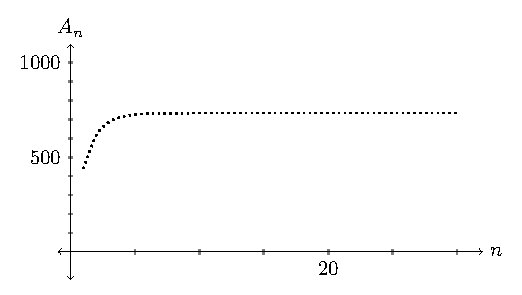
\includegraphics[width=.92\linewidth]{../figures/fhsm_2009_p46_1.pdf}
      \end{center}

      Students may observe that the level of medicine in the body initially rises rapidly but with time increases less rapidly. Thus, the rate of change of this function does not remain constant. Even a beginning student could surmise from this table that the medicine level appears to eventually stabilize, so that after about seventeen dosage periods, the value no longer seems to change. In terms of metabolism, students could explain that the athlete's body is eliminating the same amount of medication as she is taking in each dose. This observation can be mathematically verified by showing that
      $$
      0.6\left(733\frac{1}{3}\right)=440
      $$
      because the value of $A_n$ approaches a limiting value of  
      $$
      733\frac{1}{3} \, \text{mg}
      $$
      after about seventeen doses.

      \item[Method 2.] A problem such as this can be expressed in recursive notation. A recursive definition for the sequence of medicine levels in the athlete's body would be $A_{n+1} = 0.40A_n + 440$, $A_1 = 0$. Obtaining explicit formulas from tables of data is often quite difficult and in some situations, impossible. A recursive approach, especially when supported by a calculator or an electronic spreadsheet, is more intuitive and gives students access to such interesting problems as this earlier in their schooling.
      
      \item[Method 3.] Students who are studying exponential functions might use a problem such as this to develop their understanding of exponential decay. By examining the pattern of medicine levels, students can observe that the change of medicine level in the athlete's body is decreasing; specifically, each change is $40$ percent of the previous amount of change. After reasoning about the repetitive nature of multiplying by $0.4$, students could express this relationship with the explicit function
      $$
      I(n)=440(0.4^{n-1}),
      $$
      where $I(n)$ represents the increase in medicine level after dose number $n$. When students are ready, an illuminating exercise would be to verify this result formally, as follows:

      \begin{quotation}
        If a sequence $A_n$ satisfies a linear recursion $A_{n+1} = a \cdot A_n + b$ for some constants $a$ and $b$, then the differences $A_n +1 - A_n$ satisfy the simpler recursion
        \begin{align*}
          &A_{n+1}-A_n \\
          &\quad =(a\cdot A_n+b)-(a\cdot A_{n-1}+b) \\
          &\quad =a\cdot (A_n-A_{n-1}).
        \end{align*}

        Therefore, these differences are just powers of a times the first difference:
        $$
        A_{n+1}-A_n
          =a^n\cdot (A_1-A_0).
        $$
      \end{quotation}

      Note that we can show from this result that $A_n$ itself is the sum of a geometric progression. Thus, this kind of problem can provide another motivation for an application of geometric progressions.

      \item[Method 4.] For older students with a more sophisticated mathematical background, this problem could be revisited as a means of informally introducing them to the important mathematical concept of limit, especially when coupled with a discrete graph of the sequence, as shown in the graph on the previous page.
      
      \item[Method 5.] Students who have more experience with reasoning and sense making may be asked to formally justify why the level of medicine converges, thus creating a deeper understanding of the phenomenon and why it happens. In this approach to the problem, students are asked to use a formal proof to show that the sequence will converge for large numbers of doses. For instance, consider the recursive function for the amount $A$ of medicine in the athlete's body after $n$ doses:
      \begin{align*}
        A_{n+1}
          &=A_n-0.6A_n+440 \\
          &=0.4A_n+440. \tag{1}
      \end{align*} 

      We can define the behavior of the medicine level as a linear function $C$, called the \emph{transition function governing the sequence} $A_n$ , where
        \begin{align*}
          C(x)=0.4x+440. \tag{2}
        \end{align*} 
      By substitution, we can write
      \begin{align*}
        A_{n+1}
          &=0.4A_n+440 \\
          &=C(A_n). \tag{3}
      \end{align*} 

      Now if the medicine concentrations truly level off, we can let $V$ represent the fixed value approached by $A_n$ after a certain number of doses, called the \emph{fixed point of} $C$. Doing so leads to the equation\vspace{1.5\baselineskip}
      \begin{align*}
        C(V)=V, \; \text{or} \; 0.4V+440=V. \tag{4}
      \end{align*}
      Solving equation (4) for $V$ gives us the value
      $$
        V=733\frac{1}{3},
      $$
      which proves that the limiting value of the blood concentration is
      $$
        V=733\frac{1}{3} \, \text{mg}
      $$
      as explained by the transition function $C$, defined in equation (2).

      To see how the transition function guarantees the convergence, we can rewrite it to display the difference between the actual amount and the fixed value. Define $D_n$ as the difference between the actual amount of medicine, $A_n$, and the fixed value, $V$:
        \begin{align*}
          A_n=V+D_n. \tag{5}
        \end{align*} 
      Substituting this result in the recursion relation, equation (3), gives
      \begin{align*}
        A_{n+1}
          &=0.4(V+D_n)+440\\
          &=(0.4+440)+0.4D_n. \tag{6}
      \end{align*} 
      Since $A_{n+1} = V + D_{n+1}$, from equation (5), and since $V$ is defined by the relation $V = 0.4V + 440$, from equation (4), we can reduce the relationship further:
      \begin{align*}
        &V+D_{n+1} \\
        &\quad =(0.4V+440)+0.4D_n, \\
        & (0.4V+440)+0.4D_{n+1} \\
        &\quad =(0.4V+440)+0.4D_n.  
      \end{align*}
      From this result we can derive the simple recursion
        \begin{align*}
          D_{n+1}=0.4D_n, \tag{7}
        \end{align*}   
      which shows that at each step, $D_n$ shrinks to $40$ percent of its previous value. Clearly, after not too many steps, $D_n$ will become negligibly small, as was suggested by the foregoing numerical calculations.
    \end{description}\vspace{.5\baselineskip}

    \textbf{Key Mathematical Elements}

    \begin{hanglist}
      \hangitem{Reasoning with Functions---Using multiple representations of functions; Modeling by using families of functions}
      \hangitem{Reasoning with Algebraic Symbols---Meaningful use of symbols; Mindful manipulation}
    \end{hanglist}

    \textbf{Reasoning Habits}

    \begin{hanglist}
      \hangitem{Analyzing a problem---identifying relevant concepts, procedures, or representations; seeking patterns and relationships}
      \hangitem{Implementing a strategy---making logical deductions}
      \hangitem{Reflecting on a solution---justifying or validating a solution}
    \end{hanglist}
  }
  {
    Uống theo chỉ dẫn
  }
  {
    \textbf{Nhiệm vụ}

    Một học sinh bị căng khớp gối khi chơi bóng chuyền trong hoạt động thể thao nội bộ, và bác sĩ kê một loại thuốc kháng viêm để giảm sưng. Học sinh uống hai viên $220$ mg mỗi $8$ giờ trong $10$ ngày. Thận của học sinh loại bỏ $60$ phần trăm lượng thuốc này khỏi cơ thể sau mỗi $8$ giờ. Hãy xác định lượng thuốc có trong cơ thể sau $10$ ngày, ngay sau khi học sinh uống liều thuốc cuối cùng. Giải thích điều gì xảy ra đối với sự thay đổi của lượng thuốc trong cơ thể theo thời gian và vì sao mẫu hình này xuất hiện. Nếu học sinh tiếp tục uống thuốc trong một năm, thì ngay sau khi uống liều thuốc cuối cùng, lượng thuốc trong cơ thể sẽ là bao nhiêu? Hãy giải thích, theo các thuật ngữ toán học và theo cơ chế chuyển hóa của cơ thể, vì sao lượng thuốc dài hạn trong cơ thể là hợp lý (phỏng theo NCTM [2000b]).\vspace{\baselineskip}

    \textbf{Trong lớp học (Nhiều trình độ, từ Toán năm thứ nhất đến Toán năm thứ tư)}

    Học sinh có thể xem xét bài toán này ở những độ sâu khác nhau, tùy theo trải nghiệm toán học của các em:

    \begin{description}
      \item[Phương pháp 1.] Những học sinh ở giai đoạn đầu trung học phổ thông có thể lập bảng dữ liệu và vẽ đồ thị rời rạc của dữ liệu. Bảng và đồ thị sau đây cho thấy lượng thuốc $A_n$ (tính theo mg) có trong cơ thể vận động viên ngay sau khi uống $n$ liều thuốc.\vspace{\baselineskip}
      
      \begin{center}
      \setlength{\tabcolsep}{5pt}
      \begin{tabular}{|c|c|c|c|c|}
      \hline
      $n$   & $1$      & $2$      & $3$      & $4$      \\
      \hline
      $A_n$ & $440$    & $616$    & $686.40$ & $714.56$ \\
      \hline
      $n$   & $5$      & $6$      & $7$      & $8$      \\
      \hline
      $A_n$ & $725.82$ & $730.33$ & $732.13$ & $732.85$ \\
      \hline
      $n$   & $9$      & $10$     & $11$     & $12$     \\
      \hline
      $A_n$ & $733.14$ & $733.26$ & $733.30$ & $733.32$ \\
      \hline
      $n$   & $\dots$  & $20$     & $\dots$  & $30$     \\
      \hline
      $A_n$ & $\dots$  & $733.33$ & $\dots$  & $733.33$ \\
      \hline
      \end{tabular}
      \end{center}

      \begin{center}
        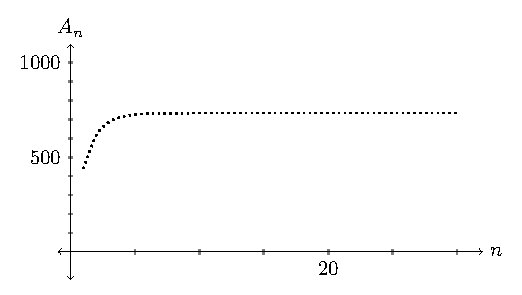
\includegraphics[width=.92\linewidth]{../figures/fhsm_2009_p46_1.pdf}
      \end{center}

      Học sinh có thể nhận thấy rằng ban đầu lượng thuốc trong cơ thể tăng nhanh, nhưng theo thời gian thì tăng chậm dần. Do đó, tốc độ thay đổi của hàm số này không giữ nguyên. Ngay cả học sinh mới bắt đầu cũng có thể phỏng đoán từ bảng rằng lượng thuốc dường như dần ổn định, đến mức sau khoảng mười bảy chu kì dùng thuốc, giá trị ấy gần như không còn thay đổi. Về mặt chuyển hóa, học sinh có thể giải thích rằng cơ thể vận động viên đang đào thải đúng bằng lượng thuốc được đưa vào ở mỗi liều. Quan sát này có thể được kiểm chứng bởi toán học bằng cách chỉ ra rằng\vspace{\baselineskip}
      $$
      0.6\left(733\frac{1}{3}\right)=440
      $$
      bởi vì $A_n$ tiến dần tới giá trị giới hạn\vspace{\baselineskip}
      $$
      733\frac{1}{3} \, \text{mg}
      $$
      sau khoảng mười bảy liều.

      \item[Phương pháp 2.] Bài toán như thế này có thể được biểu diễn bằng kí hiệu truy hồi. Một định nghĩa truy hồi cho dãy lượng thuốc trong cơ thể vận động viên là $A_{n+1}=0.40A_n+440,\, A_0=0$. Việc rút ra công thức tường minh từ bảng dữ liệu thường rất khó, và trong một số tình huống là không thể. Cách tiếp cận truy hồi, đặc biệt khi có máy tính cầm tay hoặc bảng tính điện tử hỗ trợ, thường trực quan hơn và cho phép học sinh tiếp cận những bài toán thú vị như thế này sớm hơn trong quá trình học.
      
      \item[Phương pháp 3.] Những học sinh đang học về hàm mũ có thể dùng bài toán như thế này để phát triển hiểu biết về suy giảm theo hàm mũ. Khi xem xét mẫu hình lượng thuốc, học sinh có thể quan sát thấy độ tăng lượng thuốc trong cơ thể vận động viên đang giảm dần; cụ thể, mỗi độ tăng bằng $40$ phần trăm độ tăng trước đó. Sau khi luận về tính lặp lại của việc nhân với $0.4$, học sinh có thể diễn tả quan hệ này bằng hàm số tường minh\vspace{2\baselineskip}
      $$
      I(n)=440(0.4^{n-1}),
      $$
      trong đó $I(n)$ biểu thị độ tăng lượng thuốc sau liều thứ $n$. Khi học sinh đã sẵn sàng, một bài tập có sức soi sáng là kiểm chứng kết quả này một cách hình thức như sau:
      
      \begin{quotation}
        Nếu một dãy $A_n$ thỏa mãn truy hồi tuyến tính $A_{n+1}=a\cdot A_n+b$ với các hằng số $a$ và $b$, thì các sai phân $A_{n+1}-A_n$ thỏa mãn truy hồi đơn giản hơn
        \begin{align*}
          &A_{n+1}-A_n \\
          &\quad =(a\cdot A_n+b)-(a\cdot A_{n-1}+b) \\
          &\quad =a\cdot (A_n-A_{n-1}).
        \end{align*}
        Do đó, các sai phân này chính là lũy thừa của $a$ nhân với sai phân đầu tiên:
        $$
        A_{n+1}-A_n
          =a^n\cdot (A_1-A_0).
        $$
      \end{quotation}

      Lưu ý rằng từ kết quả này, có thể suy ra bản thân $A_n$ là tổng của một cấp số nhân. Vì vậy, dạng bài toán này có thể cung cấp thêm động lực cho một ứng dụng của cấp số nhân.

      \item[Phương pháp 4.] Đối với những học sinh lớn hơn, có nền tảng toán học tinh vi hơn, bài toán này có thể được quay lại như một phương tiện để giới thiệu không chính thức khái niệm giới hạn, một khái niệm quan trọng của toán học, đặc biệt khi được đặt cùng đồ thị rời rạc của dãy như trong hình ở trang trước.
      
      \item[Phương pháp 5.] Những học sinh có nhiều trải nghiệm hơn với luận và hiểu có thể được yêu cầu biện minh một cách hình thức vì sao lượng thuốc hội tụ, qua đó hình thành sự hiểu sâu hơn về hiện tượng và lí do hiện tượng ấy xảy ra. Trong cách tiếp cận này, học sinh được yêu cầu dùng chứng minh hình thức để chỉ ra rằng dãy sẽ hội tụ khi số liều lớn. Chẳng hạn, xét hàm truy hồi cho lượng thuốc $A$ trong cơ thể vận động viên sau $n$ liều:\vspace{2\baselineskip}
      \begin{align*}
        A_{n+1}
          &=A_n-0.6A_n+440 \\
          &=0.4A_n+440. \tag{1}
      \end{align*} 

      Ta có thể mô tả hành vi của lượng thuốc bằng một hàm tuyến tính $C$, gọi là \emph{hàm chuyển tiếp chi phối dãy} $A_n$, trong đó\vspace{\baselineskip}
        \begin{align*}
          C(x)=0.4x+440. \tag{2}
        \end{align*} 
      Bằng phép thế, ta có thể viết
      \begin{align*}
        A_{n+1}
          &=0.4A_n+440 \\
          &=C(A_n). \tag{3}
      \end{align*} 

      Bây giờ, nếu lượng thuốc thật sự dần ổn định, ta có thể dùng $V$ để biểu thị giá trị cố định mà $A_n$ tiến tới sau một số liều nhất định; giá trị này được gọi là \emph{điểm bất động của} $C$. Việc này dẫn đến phương trình
      \begin{align*}
        C(V)=V, \; \text{hoặc} \; 0.4V+440=V. \tag{4}
      \end{align*}

      Giải phương trình (4) theo $V$ cho ta giá trị 
      $$
        V=733\frac{1}{3},
      $$
      chứng tỏ rằng giá trị giới hạn của lượng thuốc là\vspace{\baselineskip}
      $$
        V=733\frac{1}{3} \, \text{mg}
      $$      
      như được giải thích bởi hàm chuyển tiếp $C$ đã định nghĩa trong phương trình (2).

      Để thấy hàm chuyển tiếp bảo đảm sự hội tụ như thế nào, ta có thể viết lại hàm ấy để làm lộ độ lệch giữa lượng thuốc thực tế và giá trị cố định. Gọi $D_n$ là độ lệch giữa lượng thuốc thực tế $A_n$ và giá trị cố định $V$:
      \begin{align*}
          A_n=V+D_n. \tag{5}
      \end{align*}

      Thay kết quả này vào hệ thức truy hồi, tức phương trình (3), ta được
      \begin{align*}
        A_{n+1}
          &=0.4(V+D_n)+440\\
          &=(0.4+440)+0.4D_n. \tag{6}
      \end{align*} 

      Vì $A_{n+1}=V+D_{n+1}$ theo phương trình (5), và vì $V$ được xác định bởi hệ thức $V=0.4V+440$ theo phương trình (4), ta có thể rút gọn quan hệ này thêm nữa:
      \begin{align*}
        &V+D_{n+1} \\
        &\quad =(0.4V+440)+0.4D_n, \\
        & (0.4V+440)+0.4D_{n+1} \\
        &\quad =(0.4V+440)+0.4D_n.  
      \end{align*}

      Từ kết quả này, ta có thể suy ra truy hồi đơn giản
      \begin{align*}
          D_{n+1}=0.4D_n, \tag{7}
      \end{align*}
      cho thấy ở mỗi bước, $D_n$ giảm xuống còn $40$ phần trăm giá trị trước đó. Rõ ràng, chỉ sau không quá nhiều bước, $D_n$ sẽ trở nên nhỏ đến mức có thể xem như không đáng kể, đúng như các phép tính số ở trên đã gợi ra.
    \end{description}

    \textbf{Các yếu tố then chốt của toán học}

    \begin{hanglist}
      \hangitem{Luận với hàm số---Sử dụng nhiều biểu diễn của hàm số; Mô hình hóa bằng các họ hàm số}

      \hangitem{Luận với ký hiệu đại số---Sử dụng ký hiệu có nghĩa; Biến đổi có ý thức}
    \end{hanglist}\vspace{\baselineskip}

    \textbf{Thói quen luận}

    \begin{hanglist}
      \hangitem{Phân tích bài toán---xác định khái niệm, thủ tục hoặc biểu diễn toán học thích đáng; tìm kiếm mẫu hình và quan hệ}

      \hangitem{Triển khai chiến lược---thực hiện suy diễn logic}

      \hangitem{Phản tư về lời giải---biện minh hoặc kiểm chứng lời giải}
    \end{hanglist}
  }
  {
    \vspace{.5\baselineskip}
    Điểm cần chú ý trước hết là bài toán này có một cấu trúc rất đặc biệt: mỗi lần uống, cơ thể được đưa vào một lượng thuốc cố định, $440$ mg; nhưng lượng thuốc bị đào thải sau mỗi chu kì không cố định, vì nó bằng $60\%$ lượng thuốc đang có trong cơ thể. Khi lượng thuốc trong cơ thể còn ít, lượng đào thải cũng ít, nên tổng lượng thuốc sau mỗi liều tăng nhanh. Khi lượng thuốc đã nhiều hơn, lượng đào thải trước liều kế tiếp cũng nhiều hơn, nên phần tăng thêm sau mỗi liều nhỏ dần. Trạng thái ổn định xuất hiện khi lượng đào thải trong một chu kì đúng bằng lượng thuốc được đưa thêm vào:
    $$
    0.6V=440.
    $$

    Do đó
    $$
    V=733\frac{1}{3}\, \text{mg}.
    $$

    Nói bằng ngôn ngữ chuyển hóa, cơ thể không làm cho thuốc ``biến mất'' hoàn toàn sau mỗi chu kì; nó chỉ giữ lại $40\%$ lượng đang có. Chính sự kết hợp giữa bổ sung cố định và đào thải theo tỉ lệ làm cho lượng thuốc tiến dần tới một mức cân bằng.

    Cần lưu ý một lỗi chỉ số trong bản gốc ở Method 2. Bản gốc viết truy hồi dạng $A_{n+1}=0.40A_n+440$ kèm điều kiện đầu $A_1=0$. Nhưng ngay trong bảng số liệu, $A_n$ đã được hiểu là lượng thuốc trong cơ thể ngay sau khi uống $n$ liều. Vì vậy, sau liều thứ nhất phải có
    $$
    A_1=440,
    $$
    không thể là $0$. Điều kiện đầu đúng phải là
    $$
    A_0=0,
    $$
    nghĩa là trước khi uống liều đầu tiên, trong cơ thể chưa có lượng thuốc này. Khi đó
    $$
    A_1=0.4A_0+440=440,
    $$
    khớp với bảng dữ liệu. Nếu giữ $A_1=0$, công thức truy hồi sẽ làm lệch toàn bộ cách đánh số liều và mâu thuẫn với chính định nghĩa của $A_n$ trong bài.

    Ví dụ này cho thấy rõ giá trị của một bài toán có thể được quay lại nhiều lần ở những mức độ khác nhau của luận và hiểu. Cùng bối cảnh---thuốc được bổ sung theo chu kì và bị đào thải theo tỉ lệ cố định---có thể trước hết được đọc bằng bảng số liệu và đồ thị rời rạc để làm lộ trực giác về sự ổn định, rồi được mô hình hóa bằng hệ thức truy hồi
    $$
    A_{n+1}=0.4A_n+440,\, A_0=0.
    $$

    Sau đó, cùng mô hình ấy có thể được nhìn lại như một bài toán về suy giảm theo hàm mũ, về khái niệm giới hạn, và cuối cùng là về chứng minh hội tụ. Chính cấu trúc nhiều tầng này làm cho ví dụ trở thành trục nối giữa mô hình hóa, hàm số, biểu diễn và suy diễn logic.

    Điểm đáng chú ý nhất nằm ở sự khác nhau giữa Phương pháp 3 và Phương pháp 5. Ở Phương pháp 3, trọng tâm được chuyển sang mức tăng
    $$
    I(n)=A_n-A_{n-1}.
    $$

    Từ hệ thức truy hồi, ta có
    $$
    A_{n+1}-A_n=0.4(A_n-A_{n-1}),
    $$
    nên mỗi mức tăng mới chỉ còn $40\%$ mức tăng trước đó. Vì mức tăng ban đầu là
    $$
    A_1-A_0=440,
    $$
    nên
    $$
    I(n)=440(0.4^{n-1}).
    $$

    Cách nhìn này hiệu quả vì nó giải thích vì sao lượng thuốc tăng chậm dần: các phần tăng thêm không biến mất ngẫu nhiên, mà giảm theo một quy luật mũ. Từ đó, học sinh có thêm động lực tự nhiên để hiểu cấp số nhân và tổng của cấp số nhân trong một tình huống có nghĩa.

    Phương pháp 5 đi xa hơn vì nó xem toàn bộ quá trình dùng thuốc như một phép lặp trạng thái. Ở đây, ta chọn một mốc quan sát cố định: lượng thuốc trong cơ thể ngay sau mỗi liều. Kí hiệu $A_n$ là lượng thuốc trong cơ thể ngay sau liều thứ $n$. Khi đó, từ $A_n$ đến $A_{n+1}$, cơ thể trải qua đúng một chu kì: trong $8$ giờ tiếp theo, cơ thể đào thải $60\%$ lượng thuốc đang có, nên chỉ còn lại $40\%$, tức là $0.4A_n$; sau đó học sinh uống liều kế tiếp, thêm $440$ mg. Vì vậy,
    $$
    A_{n+1}=0.4A_n+440.
    $$

    Hàm
    $$
    C(x)=0.4x+440
    $$
    được gọi là hàm chuyển tiếp vì nó mô tả đúng một bước chuyển từ trạng thái này sang trạng thái kế tiếp: nếu lượng thuốc ngay sau một liều là $x$, thì lượng thuốc ngay sau liều kế tiếp là $C(x)$. Do đó, toàn bộ dãy lượng thuốc được tạo ra bằng cách lặp đi lặp lại cùng một hàm:
    $$
    A_{n+1}=C(A_n).
    $$

    Theo cách nhìn này, giá trị ổn định không còn chỉ là con số được đoán ra từ bảng, mà là một trạng thái không đổi qua phép chuyển tiếp. Nếu ngay sau một liều cơ thể đang có $V$ mg thuốc, và sau một chu kì đào thải rồi uống liều kế tiếp, lượng thuốc lại trở về đúng $V$ mg, thì $V$ phải thỏa
    $$
    C(V)=V.
    $$

    Nói cách khác,
    $$
    0.4V+440=V.
    $$

    Giải ra được
    $$
    V=733\frac{1}{3}\, \text{mg}.
    $$

    Đây là ý nghĩa của điểm bất động: đó là mức thuốc mà phép chuyển tiếp $C$ giữ nguyên. Nếu cơ thể đang ở đúng mức ấy ngay sau một liều, thì sau khi đào thải $60\%$ trong $8$ giờ và uống thêm $440$ mg, lượng thuốc lại trở về đúng mức ấy. Về mặt chuyển hóa, điều này tương đương với việc lượng thuốc bị đào thải trong một chu kì đúng bằng lượng thuốc được đưa thêm vào.

    Tuy nhiên, tìm được điểm bất động mới cho biết mức cân bằng là bao nhiêu; điều còn cần chứng minh là dãy $A_n$ có thật sự tiến tới mức cân bằng ấy hay không. Vì vậy, Phương pháp 5 xét độ lệch giữa lượng thuốc thực tế và mức cân bằng:
    $$
    D_n=A_n-V.
    $$

    Từ
    $$
    A_{n+1}=0.4A_n+440
    $$
    và
    $$
    V=0.4V+440,
    $$
    lấy hai đẳng thức trừ nhau, ta được
    $$
    A_{n+1}-V=0.4(A_n-V).
    $$

    Tức là
    $$
    D_{n+1}=0.4D_n.
    $$

    Do đó, sau mỗi chu kì, độ lệch so với mức cân bằng chỉ còn $40\%$ độ lệch trước đó; nói theo khoảng cách,
    $$
    \lvert D_{n+1}\rvert=0.4\lvert D_n\rvert.
    $$

    Vì $0.4<1$, các độ lệch này nhỏ dần về $0$. Đây là phần chứng minh hội tụ: lượng thuốc không chỉ có vẻ ổn định qua bảng số liệu, mà buộc phải tiến dần tới $733\frac{1}{3}$ mg do chính cấu trúc của phép lặp. Ở đây, ``ổn định'' không còn là quan sát số học từ bảng, mà trở thành hệ quả tất yếu của hàm chuyển tiếp $C$.

    Giá trị sư phạm của ví dụ vì thế không nằm riêng ở lời giải cho bài toán, mà ở cách nó cho phép cùng một tình huống nâng đỡ nhiều mức học khác nhau. Người mới học có thể bắt đầu từ bảng và đồ thị; học sinh khá hơn có thể nhận ra hệ thức truy hồi và cấu trúc mũ; học sinh đã vững vàng hơn có thể dùng điểm bất động và độ lệch để giải thích vì sao hội tụ xảy ra. Nhờ đó, ví dụ minh họa đúng tinh thần của sách: hiểu không tách rời luận, và cùng một bối cảnh tốt có thể đưa người học từ trực giác định lượng đến biện giải chặt chẽ.
  }

\TriPara
  {
    \EN{Incorporating formal proof throughout the high school mathematics curriculum serves to strengthen students' reasoning skills and can also ease the transition from high school to college mathematics. The general reasoning in example 11, ``Take As Directed,'' can be extended to a range of other situations, as shown in example 12, which demonstrates an application of formal proof to the important context of finance. This example shows how students can grow in their own reasoning ability by studying and interpreting the reasoning of others.}
  }
  {
    \VI{Việc lồng ghép chứng minh hình thức xuyên suốt chương trình toán học trung học phổ thông giúp củng cố năng lực luận của học sinh, đồng thời làm cho bước chuyển tiếp từ toán phổ thông sang toán đại học trở nên thuận lợi hơn. Mạch luận tổng quát trong Ví dụ 11, ``Uống theo chỉ dẫn'', có thể được mở rộng sang nhiều tình huống khác, như Ví dụ 12 cho thấy qua một ứng dụng của chứng minh hình thức trong bối cảnh tài chính. Ví dụ này cho thấy học sinh có thể phát triển năng lực luận của bản thân thông qua việc tìm hiểu và diễn giải mạch luận của người khác.}
  }{\NOTE{}}

\TriExample
  {
    Money Matters
  }
  {
    \textbf{Task}

    After exploring the method of formal justification in example 11 (method 5), a teacher asks her students to read and interpret the following text describing how to determine the payment amount for installment loans, and to answer a series of questions about the text.

    \begin{quote}
      When someone takes out an installment loan, we need to be able to find the monthly payment amount so that the loan is paid off in a certain number of months. The monthly payment on an installment loan includes the interest charged on the unpaid amount of the loan (the principal) since the last payment. Any amount of the payment left over after the interest is deducted goes toward paying off the loan, thereby reducing the principal.

      Let's express this situation by using algebraic notation. Define $P_n$ to be the principal owed at the end of period $n$, where $P_0$ is the amount initially borrowed. If the interest rate for a single period is r and the borrower makes a monthly payment $M$ at the end of each period, then the principal owed at the end of the period $n + 1$ can be written as $P_{n+1}=P_n+rP_n-M=(1+r)P_n-M$. Thus, the principal owed at the end of one month is related to the principal owed the month before by the linear function $P_{n+1}=Q(P_n)$, where $Q(x)=(1+r)x-M$.

      If we want to pay the principal off in $m$ months, then $P_m = 0$. Noting that $P_m=Q(P_m-1) =Q(Q(P_{m-2})) = Q(Q(Q(P_{m-3})))$, and so forth, we can see that $P_m = Q^{(m)}(P_0) = 0$, where we use $Q^{(m)}$ to stand for the composition of $Q$ with itself m times. If we can find an expression for $Q^{(m)}(P_0)$ in terms of $P_0$, $M$, $m$, and $r$, we can solve the equation $Q^{(m)}(P_0) = 0$ for $M$ in terms of the given variables.

      However, finding the expression is not easy. We can use a fixed-point analysis to simplify the effect of $Q$. If $F$ is the fixed point of $Q$, then $Q(F) = F$. Thus, $Q(F)=(1+r)F-M = F$. So we can see that $F = M/r$.\vspace{\baselineskip}

      Next, let us define $D_n$ as the difference between $P_n$ and the fixed point $F$, that is,
      $$
        D_n=P_n-F, \; \text{or} \; P_n=F+D_n.
      $$

      Then, on the one hand,
      \begin{align*}
        Q(P_n)
          &=Q(F+D_n) \\
            & \text{(from our definition of $D_n$)} \\
          &=(1+r)(F+D_n)-M \\
            & \text{(by applying the definition of $Q$)} \\
          &=((1 + r)F - M) + (1 + r)D_n \\
            & \text{(by distribution and} \\
            & \text{rearranging terms)} \\
          &=Q(F) + (1 + r)D_n \\
            & \text{(again by applying} \\
            & \text{the definition of $Q$)} \\
          &=F + (1 + r)D_n \\
            & \text{(since $F$ is the fixed point for $Q$).}
      \end{align*}

      On the other hand,
      \begin{align*}
        Q(P_n)
          &=P_{n+1} \\
            & \text{(by definition of $Q$)} \\
          &=F + D_{n+1} \\
            & \text{(by definition of $D_{n+1}$).}
      \end{align*}

      Equating the two expressions for $Q(P_n)$ gives
      \begin{align*}
        F+(1+r)D_n&=F+D_{n+1}, \, \text{or} \\
        D_{n+1}&=(1+r)D_n.
      \end{align*}

      Thus, $D_n$ , the difference between $P_n$ and the fixed point $F$, varies in a simpler way than $P_n$ does: it is simply multiplied by $(1 + r)$ at each step.

      Applying this relation twice gives
      \begin{align*}
        D_{n+2}
          &=(1+r)D_{n+1} \\
            & \text{(by substituting $n + 1$ for $n$)} \\
          &=(1+r)((1+r)D_n) \\
            & \text{(by the equation for $n$)} \\
          &=(1+r)^2D_n \\
            & \text{(by the associative rule and} \\
            & \text{the definition of exponents).}
      \end{align*}

      Iterating this reasoning gives us the relation
      $$
        D_m = (1 + r)^m D_0.
      $$

      If we rewrite this result in terms of $P_m$, we find
      \begin{align*}
        P_m
          &=F+D_m \\
          &=F+(1+r)^mD_0 \\
          &=F+(1+r)^m(P_0-F) \\
          &=(1+r)^mP_0+F\left(1-(1+r)^m\right).
      \end{align*}

      By using the formula $F = M/r$, we get
      $$
        P_m=(1+r)^mP_0+(M/r)\left(1-(1+r)^m\right),
      $$
      which is the expression we were looking for. By setting $P_m = 0$, we can now solve for $M$:
      $$
        M=r\cdot P_0\cdot \frac{(1+r)^m}{(1+r)^m-1}.
      $$
    \end{quote}\vspace{.35\baselineskip}

    \textbf{\emph{Answer the following questions about this analysis:}}

    \begin{enumerate}
      \item How does the function describing the successive periods of an installment loan compare with the function describing the blood concentrations in successive periods when taking a medicine?
      
      \item Compare the effect of $Q$ in this situation and $C$ in the medicine problem, example 11. Why do we want to find a fixed point in each situation?\vspace{\baselineskip}
      
      \item How does the multiplier $(1 + r)$ differ between this situation and the medicine problem, example 11? How does the value of the multiplier ensure that we can eventually pay off the loan?
      
      \item Explain how the underlying mathematics in this situation is very similar to finding the blood concentration of medicine, even though the two situations appear very different. 
    \end{enumerate}

    \textbf{Key Mathematical Elements}

    \begin{hanglist}
      \hangitem{Reasoning with Functions---Modeling by using families of functions}

      \hangitem{Reasoning with Algebraic Symbols---Mindful manipulation; Reasoned solving}
    \end{hanglist}

    \textbf{Reasoning Habits}

    \begin{hanglist}
      \hangitem{Analyzing a problem---defining relevant variables and conditions}

      \hangitem{Implementing a strategy---making logical deductions}
      
      \hangitem{Reflecting on a solution---reconciling different approaches; generalizing a solution}
    \end{hanglist}
  }
  {
    Chuyện tiền bạc
  }
  {
    \textbf{Nhiệm vụ}

    Sau khi tìm hiểu phương pháp biện minh hình thức trong Ví dụ 11 (Phương pháp 5), giáo viên yêu cầu học sinh đọc và diễn giải đoạn văn sau, trong đó mô tả cách xác định khoản thanh toán cho một khoản vay trả góp, rồi trả lời một loạt câu hỏi về đoạn văn ấy.

    \begin{quote}  
      Khi một người vay tiền theo hình thức trả góp, ta cần xác định khoản phải trả hằng tháng sao cho khoản vay được trả hết sau một số tháng nhất định. Khoản thanh toán hằng tháng của khoản vay trả góp bao gồm phần lãi tính trên số tiền vay còn chưa trả, tức tiền gốc, kể từ lần thanh toán trước. Phần còn lại của khoản thanh toán sau khi trừ lãi sẽ được dùng để trả bớt khoản vay, nhờ đó làm giảm tiền gốc.\vspace{\baselineskip}

      Hãy diễn tả tình huống này bằng kí hiệu đại số. Gọi $P_n$ là tiền gốc còn nợ vào cuối kì thứ $n$, trong đó $P_0$ là số tiền vay ban đầu. Nếu lãi suất cho một kì là $r$ và người vay trả khoản $M$ vào cuối mỗi kì, thì tiền gốc còn nợ vào cuối kì thứ $n+1$ có thể được viết là $P_{n+1}=P_n+rP_n-M=(1+r)P_n-M$. Vì thế, tiền gốc còn nợ vào cuối một tháng liên hệ với tiền gốc còn nợ cuối tháng trước qua hàm tuyến tính $P_{n+1}=Q(P_n)$, trong đó $Q(x)=(1+r)x-M$.\vspace{3\baselineskip}

      Nếu ta muốn trả hết tiền gốc trong $m$ tháng, thì $P_m=0$. Nhận thấy rằng $P_m=Q(P_{m-1})=Q(Q(P_{m-2}))=Q(Q(Q(P_{m-3})))$, vân vân, ta có thể thấy rằng $P_m=Q^{(m)}(P_0)=0$, trong đó $Q^{(m)}$ kí hiệu phép hợp thành $Q$ với chính nó $m$ lần. Nếu tìm được biểu thức cho $Q^{(m)}(P_0)$ theo $P_0$, $M$, $m$, và $r$, thì ta có thể giải phương trình $Q^{(m)}(P_0)=0$ để tìm $M$ theo các biến đã cho.

      Tuy nhiên, việc tìm biểu thức ấy không dễ. Ta có thể dùng phân tích điểm bất động để đơn giản hóa tác động của $Q$. Nếu $F$ là điểm bất động của $Q$, thì $Q(F)=F$. Do đó, $Q(F)=(1+r)F-M=F$. Từ đây, ta thấy $F=M/r$.

      Tiếp theo, gọi $D_n$ là độ lệch giữa $P_n$ và điểm bất động $F$, tức là
      $$
        D_n=P_n-F, \; \text{hoặc} \; P_n=F+D_n.
      $$

      Một mặt,
      \begin{align*}
      Q(P_n)
        &=Q(F+D_n) \\
          & \text{(theo định nghĩa của ta cho $D_n$)} \\
        &=(1+r)(F+D_n)-M \\
          & \text{(áp dụng định nghĩa của $Q$)} \\
        &=((1+r)F-M)+(1+r)D_n \\
          & \text{(phân phối và} \\
          & \text{sắp xếp lại các số hạng)} \\
        &=Q(F)+(1+r)D_n \\
          & \text{(lần nữa áp dụng} \\
          & \text{định nghĩa của $Q$)} \\
        &=F+(1+r)D_n \\
          & \text{(vì $F$ là điểm bất động của $Q$).}
      \end{align*}

      Mặt khác,
      \begin{align*}
      Q(P_n)
        &=P_{n+1} \\
          & \text{(theo định nghĩa của $Q$)} \\
        &=F+D_{n+1} \\
          & \text{(theo định nghĩa của $D_{n+1}$).}
      \end{align*}

      Đặt hai biểu thức của $Q(P_n)$ bằng nhau, ta được
      \begin{align*}
        F+(1+r)D_n&=F+D_{n+1}, \, \text{hay}\\
        D_{n+1}&=(1+r)D_n.
      \end{align*}

      Như vậy, $D_n$, độ lệch giữa $P_n$ và điểm bất động $F$, biến thiên theo cách đơn giản hơn $P_n$: ở mỗi bước, nó chỉ được nhân với $(1+r)$.\vspace{\baselineskip}

      Áp dụng hệ thức này hai lần cho ta\vspace{\baselineskip}
      \begin{align*}
        D_{n+2}
          &=(1+r)D_{n+1} \\
            & \text{(thay $n+1$ cho $n$)} \\
          &=(1+r)((1+r)D_n) \\
            & \text{(theo công thức với $n$)} \\
          &=(1+r)^2D_n \\
            & \text{(theo quy tắc kết hợp và} \\
            & \text{định nghĩa lũy thừa).}
      \end{align*}

      Lặp lại mạch luận này cho ta hệ thức
      $$
        D_m = (1 + r)^m D_0.
      $$

      Nếu viết lại kết quả này theo $P_m$, ta được
      \begin{align*}
      P_m
        &=F+D_m \\
        &=F+(1+r)^mD_0 \\
        &=F+(1+r)^m(P_0-F) \\
        &=(1+r)^mP_0+F\left(1-(1+r)^m\right).
      \end{align*}

      Dùng công thức $F=M/r$, ta được\vspace{\baselineskip}
      $$
        P_m=(1+r)^mP_0+(M/r)\left(1-(1+r)^m\right),
      $$
      đây chính là biểu thức cần tìm. Bây giờ, đặt $P_m=0$, ta có thể giải ra $M$:
      $$
        M=r\cdot P_0\cdot \frac{(1+r)^m}{(1+r)^m-1}.
      $$
    \end{quote}

    \textbf{\emph{Hãy trả lời các câu hỏi sau đây về phân tích này:}}

    \begin{enumerate}
      \item Hàm mô tả các kì liên tiếp của một khoản vay trả góp giống và khác gì với hàm mô tả lượng thuốc trong cơ thể ở các kì liên tiếp khi dùng thuốc?\vspace{\baselineskip}
      
      \item Hãy so sánh tác động của $Q$ trong tình huống này với tác động của $C$ trong bài toán thuốc ở Ví dụ 11. Vì sao trong mỗi tình huống ta đều muốn tìm một điểm bất động?
      
      \item Số nhân $(1+r)$ trong tình huống này khác với số nhân trong bài toán thuốc ở Ví dụ 11 như thế nào? Giá trị của số nhân này bảo đảm khả năng trả hết khoản vay ra sao?\vspace{\baselineskip}
      
      \item giải thích vì sao cấu trúc toán học nền tảng của tình huống này rất giống với bài toán tìm lượng thuốc trong cơ thể, mặc dù bề ngoài hai tình huống rất khác nhau.
    \end{enumerate}\vspace{\baselineskip}

    \textbf{Các yếu tố then chốt của toán học}

    \begin{hanglist}
      \hangitem{Luận với hàm số---Mô hình hóa bằng các họ hàm số}

      \hangitem{Luận với kí hiệu đại số---Biến đổi có ý thức; Giải có cơ sở luận}
    \end{hanglist}

    \textbf{Thói quen luận}

    \begin{hanglist}
      \hangitem{Phân tích bài toán---xác định cẩn thận biến và điều kiện thích đáng}

      \hangitem{Triển khai chiến lược---thực hiện suy diễn logic}

      \hangitem{Phản tư về lời giải---dung hòa những cách tiếp cận khác nhau; khái quát hóa lời giải}
    \end{hanglist}
  }
  {
    \vspace{.5\baselineskip}
    Ví dụ 12 nên được đọc như một phần nối tiếp tự nhiên của Ví dụ 11. Ở Ví dụ 11, lượng thuốc trong cơ thể sau mỗi liều được mô tả bằng một hàm chuyển tiếp tuyến tính: biết trạng thái hiện tại, hàm cho biết trạng thái kế tiếp. Ở đây, khoản vay trả góp cũng có cấu trúc tương tự. Nếu $P_n$ là số tiền gốc còn nợ sau kì thứ $n$, thì sau một kì, khoản nợ trước hết tăng lên do lãi, thành $(1+r)P_n$, rồi giảm đi vì người vay trả một khoản cố định $M$. Vì vậy,
    $$
    P_{n+1}=(1+r)P_n-M.
    $$

    Hàm chuyển tiếp của bài toán là
    $$
    Q(x)=(1+r)x-M.
    $$

    Nó cho biết: nếu sau một kì nào đó còn nợ $x$, thì sau kì kế tiếp, sau khi cộng lãi và trừ khoản trả, số tiền còn nợ là $Q(x)$. Như vậy, điểm chung giữa bài toán thuốc và bài toán vay là cả hai đều được tổ chức bởi một hàm chuyển tiếp tuyến tính; điểm khác là trong bài toán thuốc, hệ số nhân nhỏ hơn $1$, còn trong bài toán vay, hệ số nhân lớn hơn $1$.

    Ý tưởng điểm bất động xuất hiện vì ta muốn tìm một mốc làm cho phép lặp trở nên dễ hiểu hơn. Điểm bất động của $Q$ là giá trị $F$ thỏa
    $$
    Q(F)=F.
    $$

    Nghĩa là nếu khoản nợ đang đúng bằng $F$, thì sau khi cộng lãi và trả $M$, khoản nợ vẫn trở lại đúng bằng $F$. Từ
    $$
    (1+r)F-M=F,
    $$
    suy ra
    $$
    rF=M,
    $$
    nên
    $$
    F=\frac{M}{r}.
    $$
    
    Về tài chính, $F$ là mức nợ mà tiền lãi trong một kì đúng bằng khoản trả $M$. Nếu nợ đúng $F$, thì mỗi kì trả $M$ chỉ vừa đủ trả lãi, còn tiền gốc không giảm. Vì vậy, trong bài toán vay, điểm bất động không nên hiểu là đích mà khoản nợ sẽ tiến tới; nó là một mốc cân bằng giả định, giúp ta đo độ lệch của khoản nợ so với mốc ấy.

    Đây là điểm khác biệt quan trọng với Ví dụ 11. Trong bài toán thuốc, hệ số của hàm chuyển tiếp là $0.4<1$, nên mỗi lần lặp, độ lệch so với điểm bất động bị thu nhỏ; vì thế lượng thuốc tiến dần tới điểm bất động. Trong bài toán vay, hệ số của hàm chuyển tiếp là $1+r>1$, nên độ lệch so với điểm bất động không bị thu nhỏ mà bị phóng đại. Tuy nhiên, chính việc xét độ lệch ấy lại làm bài toán trở nên sáng rõ. Đặt
    $$
    D_n=P_n-F.
    $$

    Vì
    $$
    P_{n+1}=(1+r)P_n-M
    $$
    và
    $$
    F=(1+r)F-M,
    $$
    lấy hai đẳng thức trừ nhau, ta được
    $$
    P_{n+1}-F=(1+r)(P_n-F).
    $$
    
    Tức là
    $$
    D_{n+1}=(1+r)D_n.
    $$

    Như vậy, thay vì phải theo dõi trực tiếp một truy hồi có cả phép nhân và phép trừ, ta chỉ cần theo dõi độ lệch $D_n$, vốn biến đổi theo một quy luật nhân rất đơn giản:
    $$
    D_m=(1+r)^mD_0.
    $$

    Từ đây suy ra
    $$
    P_m-F=(1+r)^m(P_0-F).
    $$

    Do đó
    $$
    P_m=F+(1+r)^m(P_0-F).
    $$
    Thay $F=\frac{M}{r}$ vào, ta được
    $$
    P_m=\frac{M}{r}+(1+r)^m\left(P_0-\frac{M}{r}\right).
    $$

    Nếu muốn khoản vay được trả hết sau đúng $m$ kì, ta đặt $P_m=0$. Khi đó
    $$
    0=\frac{M}{r}+(1+r)^m\left(P_0-\frac{M}{r}\right).
    $$

    Giải phương trình này theo $M$ cho ta
    $$
    M=rP_0\cdot \frac{(1+r)^m}{(1+r)^m-1}.
    $$

    Đây chính là công thức khoản trả cố định mỗi kì cho một khoản vay trả góp.

    Công thức này cũng có ý nghĩa tài chính rõ ràng. Khoản trả $M$ phải đủ lớn hơn tiền lãi phát sinh ở mỗi kì để phần dư làm giảm tiền gốc. Nếu $M$ quá nhỏ, khoản nợ không giảm đủ nhanh, thậm chí có thể không giảm. Nếu chọn đúng $M$ theo công thức trên, thì quá trình cộng lãi rồi trả tiền sẽ đưa khoản nợ về $0$ sau đúng $m$ kì. Nói cách khác, công thức không chỉ là kết quả biến đổi đại số; nó mô tả sự cân bằng giữa ba đại lượng: số tiền vay ban đầu $P_0$, lãi suất mỗi kì $r$, và số kì trả nợ $m$.

    Giá trị sư phạm của ví dụ nằm ở chỗ nó cho thấy cùng một cấu trúc toán học có thể giải thích những hiện tượng rất khác nhau. Bài toán thuốc và bài toán vay đều có dạng chung
    $$
    X_{n+1}=aX_n+b.
    $$
    Khi tìm điểm bất động $F$ rồi xét độ lệch $D_n=X_n-F$, truy hồi trở thành
    $$
    D_{n+1}=aD_n.
    $$
    Trong bài toán thuốc, $|a|<1$, nên độ lệch nhỏ dần và hệ tiến về cân bằng. Trong bài toán vay, $a=1+r>1$, nên điểm bất động không phải là điểm hút; nhưng chính mốc ấy vẫn giúp biến bài toán trả góp thành một quy luật nhân đơn giản, từ đó tìm được khoản trả cần thiết. Đây là chỗ Ví dụ 12 mở rộng ý nghĩa của Ví dụ 11: một kĩ thuật đại số không chỉ dùng để chứng minh hội tụ, mà còn dùng để thiết kế một quá trình sao cho đạt được trạng thái mong muốn sau số bước định trước.

    Theo nghĩa đó, bốn câu hỏi cuối ví dụ đều quy về một ý: cần nhận ra sự tương đồng cấu trúc giữa hai tình huống, đồng thời không được đồng nhất ý nghĩa của chúng. Cùng là hàm chuyển tiếp tuyến tính, nhưng hệ số nhỏ hơn $1$ trong bài toán thuốc tạo ra sự ổn định dài hạn, còn hệ số lớn hơn $1$ trong bài toán vay buộc ta chọn khoản trả $M$ thích hợp để khoản nợ đi về $0$. Sự hiểu ở đây không nằm ở việc nhớ công thức trả góp, mà ở việc thấy vì sao điểm bất động và độ lệch là công cụ chung để đọc, giải thích và điều khiển một quá trình lặp.
  }

\ParallelSection
  {Analyzing the effects of parameters}
  {Phân tích ảnh hưởng của tham số}
  {}

\TriPara
  {
    \EN{Different but equivalent algebraic expressions can be used to define the same function, often revealing different properties of the function. For example, writing a quadratic function in the form $y = ax^2 + bx + c$ helps us identify the y-axis intercept, whereas using the form
    $$
    y=\left(\frac{1}{4p}\right)(x-h)^2+k
    $$
    enables us to quickly determine the vertex, $(h, k)$, of the parabolic graph and the location of its focus, where $p$ represents the distance from the vertex to the focus. In example 13, students make conjectures about the effects of changes to the values of parameters in a sinusoidal function and consider the reasonableness of their solution.}
  }
  {
    \VI{Những biểu thức đại số khác nhau nhưng tương đương có thể được dùng để xác định cùng một hàm số, và thường làm lộ những tính chất khác nhau của hàm số đó. Chẳng hạn, viết hàm bậc hai dưới dạng $y = ax^2 + bx + c$ giúp ta nhận diện giao điểm với trục $y$, trong khi dùng dạng
    $$
    y=\left(\frac{1}{4p}\right)(x-h)^2+k
    $$
    cho phép ta nhanh chóng xác định đỉnh $(h, k)$ của đồ thị parabol và vị trí tiêu điểm của nó, trong đó $p$ biểu thị khoảng cách từ đỉnh đến tiêu điểm. Trong Ví dụ 13, học sinh đưa ra phỏng đoán về ảnh hưởng của việc thay đổi giá trị tham số trong một hàm số hình sin và xem xét tính hợp lí của lời giải.}
  }{\NOTE{}}

\TriExample
  {Tidal Waves}
  {
    \textbf{Task}

    The captain of a shipping vessel must consider the tides when entering a seaport because the water depth can vary greatly from one time of day to another. Suppose that high tide in a certain port occurs at 5:00 a.m., when the water is $10.6$ meters deep, and the next low tide occurs at 11:00 a.m., when the water is $6.5$ meters deep. Develop a mathematical model that will predict the water depth as a function of the elapsed time since midnight.

    \textbf{In the Classroom (Fourth-Year Mathematics)}

    Note that the students working on this problem have had experience with transformations of linear and quadratic functions and are familiar with the graphs of the sine and cosine functions.

    An example of students' reasoning about this task follows:

    \begin{scriptlist}
      \item [Teacher:] We have only been given two ordered pairs, so there are many types of graphs that could fit our data. What type of algebraic model would make sense in this situation?
      
      \item [Student 1:] Two points determine a line, right? Couldn't we just connect the two points?\vspace{\baselineskip}
      
      \item [Student 2:] No, the water level doesn't just keep going down forever---it goes back up again and then down again every day.
      
      \item [Student 3:] That means it's probably going to be one of those wave-shaped graphs.
      
      \item [Student 1:] Oh, yeah---I'll bet it's going to be sine or cosine. But how do we know which one?
      
      \item [Student 3:] Well, let's try drawing part of the wave and see what we can figure out.
      
      \item [Student 2:] If the pattern repeats like this every six hours, then there will be two high points and two low points every day. I suppose that makes the period 12 hours.

      \begin{center}
        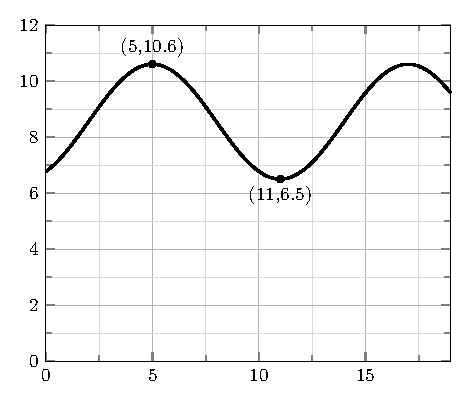
\includegraphics[width=.92\linewidth]{../figures/fhsm_2009_p52_1.pdf}
      \end{center}

      \item [Student 3:] Yeah, and if the highest and lowest the graph ever goes are $10.6$ meters and $6.5$ meters, then the amplitude is going to be $4.1$ meters, right? Oh, wait a minute---the amplitude is only half of the height, so we need to change that to $2.05$ meters.
      
      \item [Student 2:] OK, now once we know that, we can find out that the vertical shift is half way between the high and low points, which would make it $8.55$ meters.
      
      \item [Teacher:] Good job so far---now you just need to work on the period and horizontal shift. Do you think it would be easier to work with sine or cosine?\vspace{\baselineskip}
      
      \item [Student 1:] I like cosine better for this graph because we can see that a high point happens five hours after midnight, so that will make it easy to find the horizontal shift.
    \end{scriptlist}

    The conversation could continue like this in small groups, followed by a whole-class discussion of the observations made by various groups. Students could check the reasonableness of their solutions by using a dynamic graphing utility. An interesting extension of this task would be to use the model to determine the times during which a ship with a certain depth requirement would be able to safely navigate into and out of the port.

    \textbf{Key Elements of Mathematics}

    \begin{hanglist}
      \hangitem{Reasoning with Functions---Modeling by using families of functions; Analyzing the effects of parameters}
    \end{hanglist}

    \textbf{Reasoning Habits}

    \begin{hanglist}
      \hangitem{Analyzing a problem---applying previously learned concepts; making preliminary deductions and conjectures}
      
      \hangitem{Reflecting on a solution---considering the reasonableness of a solution}
    \end{hanglist}
  }
  {
    Thủy triều
  }
  {
    \textbf{Nhiệm vụ}

    Thuyền trưởng một con tàu phải tính đến thủy triều khi đưa tàu vào cảng biển, vì độ sâu của nước có thể thay đổi rất nhiều giữa các thời điểm trong ngày. Giả sử triều cao tại một cảng xảy ra lúc 5 giờ sáng, khi nước sâu $10.6$ mét, và lần triều thấp tiếp theo xảy ra lúc 11 giờ sáng, khi nước sâu $6.5$ mét. Hãy xây dựng mô hình toán học dự đoán độ sâu của nước theo thời gian đã trôi qua kể từ nửa đêm.\vspace{\baselineskip}

    \textbf{Trong lớp học (Toán năm thứ tư)}\vspace{\baselineskip}

    Lưu ý rằng học sinh làm bài toán này đã có kinh nghiệm với các phép biến đổi của hàm tuyến tính và hàm bậc hai, đồng thời quen thuộc với đồ thị của hàm sin và hàm cosin.\vspace{\baselineskip}

    Sau đây là một ví dụ về cách học sinh luận về nhiệm vụ này:

    \begin{scriptlist}
      \item [Giáo viên:] Ta chỉ được cho hai cặp có thứ tự, nên có nhiều kiểu đồ thị khác nhau có thể khớp với dữ liệu của ta. Kiểu mô hình đại số nào là hợp lí trong tình huống này?
      
      \item [Học sinh 1:] Hai điểm xác định một đường thẳng, đúng không ạ? Chẳng phải ta chỉ cần nối hai điểm đó sao?
      
      \item [Học sinh 2:] Không, mực nước đâu chỉ cứ giảm mãi---nó lại dâng lên rồi hạ xuống mỗi ngày.\vspace{\baselineskip}
      
      \item [Học sinh 3:] Điều đó có nghĩa là có lẽ đồ thị sẽ thuộc dạng sóng.\vspace{\baselineskip}
      
      \item [Học sinh 1:] À đúng rồi---em đoán nó sẽ là sin hoặc cosin. Nhưng làm sao biết nên chọn cái nào?
      
      \item [Học sinh 3:] Thử vẽ một phần đồ thị sóng rồi xem ta có thể nhận ra điều gì.
      
      \item [Học sinh 2:] Nếu mẫu hình này lặp lại như vậy sau mỗi sáu giờ, thì mỗi ngày sẽ có hai điểm cao và hai điểm thấp. Em đoán chu kì là $12$ giờ.\vspace{\baselineskip}

      \begin{center}
        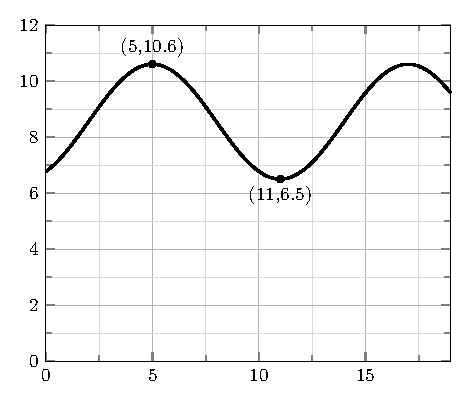
\includegraphics[width=.92\linewidth]{../figures/fhsm_2009_p52_1.pdf}
      \end{center}

      \item [Học sinh 3:] Vâng, và nếu giá trị cao nhất và thấp nhất mà đồ thị đạt tới là $10.6$ mét và $6.5$ mét, thì biên độ sẽ là $4.1$ mét, đúng không ạ? À, khoan đã---biên độ chỉ bằng một nửa độ chênh đó, nên ta cần đổi thành $2.05$ mét.\vspace{2\baselineskip}
      
      \item [Học sinh 2:] Ổn rồi, bây giờ khi đã biết điều đó, ta có thể tìm được độ dời theo phương đứng: nó nằm ở chính giữa điểm cao và điểm thấp, nên bằng $8.55$ mét.

      \item [Giáo viên:] Tốt lắm---bây giờ các em chỉ còn phải xử lí chu kì và độ dời theo phương ngang. Các em nghĩ làm việc với sin hay cosin sẽ dễ hơn?\vspace{\baselineskip}
      
      \item [Học sinh 1:] Em thích cosin cho đồ thị này hơn, vì ta có thể thấy một điểm cao xuất hiện năm giờ sau nửa đêm, nên sẽ dễ tìm độ dời theo phương ngang hơn.\vspace{\baselineskip}
    \end{scriptlist}

    Cuộc trao đổi có thể tiếp tục theo cách này trong các nhóm nhỏ, rồi sau đó là thảo luận toàn lớp về những quan sát mà các nhóm đưa ra. Học sinh có thể kiểm tra tính hợp lí của lời giải bằng cách dùng một công cụ vẽ đồ thị động. Một hướng mở rộng thú vị của nhiệm vụ này là dùng mô hình để xác định những khoảng thời gian mà một con tàu có yêu cầu nhất định về độ sâu có thể ra vào cảng an toàn.

    \textbf{Các yếu tố then chốt của toán học}

    \begin{hanglist}
      \hangitem{Luận với hàm số---Mô hình hóa bằng các họ hàm số; Phân tích ảnh hưởng của tham số}
    \end{hanglist}\vspace{\baselineskip}

    \textbf{Các thói quen luận}

    \begin{hanglist}
      \hangitem{Phân tích bài toán---vận dụng khái niệm đã học; đưa ra suy diễn và phỏng đoán sơ bộ}\vspace{\baselineskip}

      \hangitem{Phản tư về lời giải---xem xét tính hợp lí của lời giải}
    \end{hanglist}
  }
  {
    Ví dụ này đáng chú ý ở chỗ học sinh không bắt đầu từ công thức có sẵn, mà từ tình huống thực tế rồi từng bước chọn ra họ hàm thích hợp và xác định các tham số của mô hình. Vì vậy, trọng tâm của ví dụ không nằm ở việc nhớ công thức của sin hay cosin, mà ở việc đọc ra từ ngữ cảnh thông tin thật sự quyết định đối với mô hình.

    Điểm xuất phát của cuộc trao đổi là nhận xét quan trọng: chỉ với hai cặp có thứ tự thì về mặt hình thức có thể có rất nhiều đồ thị đi qua hai điểm ấy. Bởi thế, muốn chọn được mô hình hợp lí, không thể chỉ bám vào dữ liệu rời rạc, mà phải bám vào bản thân tình huống. Ở đây, học sinh nhận ra mực nước không thể cứ hạ xuống mãi; nó lên rồi xuống theo nhịp tuần hoàn. Chính ngữ cảnh thủy triều buộc người học rời khỏi ý tưởng nối hai điểm bằng đường thẳng để chuyển sang ý tưởng dùng đồ thị tuần hoàn. Đây là bước luận đầu tiên, và cũng là bước quyết định: mô hình không được chọn chỉ vì khớp với dữ liệu đã cho, mà vì phù hợp với bản chất của hiện tượng.

    Chỗ then chốt tiếp theo là cách xây dựng mô hình cosin. Từ hình vẽ, học sinh biết mực nước cao nhất là $10.6$ mét vào lúc $5$ giờ sáng, còn lần triều thấp kế tiếp là $6.5$ mét vào lúc $11$ giờ sáng. Khoảng thời gian từ một điểm cực đại đến điểm cực tiểu kế tiếp là $6$ giờ; mà đối với đồ thị sin hay cosin, khoảng ấy bằng nửa chu kì. Vì vậy, chu kì của mô hình phải là
    $$
    T=12\; \text{(giờ)}.
    $$

    Sau đó, học sinh cần phân biệt hai đại lượng rất dễ nhầm: độ chênh từ cực đại đến cực tiểu và biên độ. Hiệu giữa giá trị lớn nhất và thấp nhất là
    $$
    10.6-6.5=4.1\; \text{(mét)}.
    $$

    Nhưng $4.1$ chưa phải là biên độ; đó là toàn bộ độ chênh từ đỉnh xuống đáy. Biên độ chỉ bằng một nửa độ chênh ấy, nên
    $$
    A=\frac{10.6-6.5}{2}=2.05\; \text{(mét)}.
    $$

    Nhận xét ``à, khoan đã---biên độ chỉ bằng một nửa'' trong lời thoại làm lộ ra đúng chỗ học sinh thường nhầm, đồng thời cho thấy hiểu không xuất hiện ngay tức thì, mà được hình thành qua sửa sai.

    Tiếp theo là mức trung bình của dao động. Vì đồ thị dao động đối xứng quanh một mức giữa, nên mức này nằm chính giữa điểm cao nhất và điểm thấp nhất. Do đó,
    $$
    d=\frac{10.6+6.5}{2}=8.55\; \text{(mét)}.
    $$

    Số $8.55$ không phải một bước tính phụ thêm, mà là độ sâu trung bình quanh đó thủy triều dao động lên xuống. Chính vì thế nó trở thành tham số dời theo phương đứng của đồ thị.

    Lúc này, học sinh phải quyết định dùng sin hay cosin. Việc chọn cosin trong ví dụ không phải ngẫu nhiên. Hàm cosin ở dạng chuẩn đạt giá trị lớn nhất ngay tại điểm bắt đầu chu kì, nên khi biết đỉnh của đồ thị xảy ra tại $t=5$, việc dùng cosin làm cho mô hình hiện ra khá tự nhiên: chỉ cần dịch đồ thị sang phải $5$ đơn vị. Nếu dùng sin thì vẫn có thể làm được, nhưng phải xử lí thêm độ lệch pha một phần tư chu kì. Vì vậy, cosin là lựa chọn sáng hơn trong tình huống này.

    Từ đó, mô hình có thể được viết dưới dạng
    $$
    D(t)=A\cos\bigl(B(t-5)\bigr)+d,
    $$
    trong đó $t$ là số giờ tính từ nửa đêm, $A=2.05$, $d=8.55$, còn
    $$
    B=\frac{2\pi}{T}=\frac{2\pi}{12}=\frac{\pi}{6}.
    $$

    Suy ra
    $$
    D(t)=2.05\cos\left(\frac{\pi}{6}(t-5)\right)+8.55.
    $$

    Công thức này không rơi từ trên xuống; mỗi tham số trong nó đều được rút ra từ một đặc điểm đã đọc được trong tình huống: $2.05$ từ biên độ, $8.55$ từ mức trung bình, $12$ từ chu kì, và $5$ từ thời điểm triều cao. Điểm đẹp của ví dụ nằm ở đó: học sinh không chỉ học cách lắp số vào mẫu hình có sẵn, mà học cách đọc một hiện tượng tuần hoàn và chuyển dần những đặc điểm quan sát được của nó thành các tham số của một hàm số. Vì vậy, việc xây dựng mô hình cosin ở đây cho thấy rất rõ rằng luận với hàm số không chỉ là thao tác trên kí hiệu, mà là sự qua lại giữa ngữ cảnh thực, đồ thị và biểu thức đại số.
  }

\TriPara
  {
    \EN{Opportunities to reason with functions and use them to model real-world situations arise at every stage of a high school student's mathematical development. Providing students with varied experiences involving functions can help them internalize the sometimes confusing mathematical language of function notation (Chazan and Yerushalmy 2003; Coulombe and Berenson 2001). The development of reasoning with functions is one of the cornerstones on which a well-developed understanding of mathematics is built.}
  }
  {
    \VI{Cơ hội để luận với hàm số và dùng hàm số để mô hình hóa tình huống thực tế xuất hiện ở mọi giai đoạn trong quá trình phát triển toán học của học sinh trung học phổ thông. Việc tạo cho học sinh những trải nghiệm đa dạng liên quan đến hàm số có thể giúp các em nội hóa ngôn ngữ toán học đôi khi gây lúng túng của kí hiệu hàm (Chazan and Yerushalmy 2003; Coulombe and Berenson 2001). Việc phát triển năng lực luận với hàm số là một trong những nền tảng để xây dựng nền hiểu biết toán học vững chắc.}
  }{\NOTE{}}

\CloseGrid